En el presente estudio trabajaremos únicamente con grafos simples, así que de ahora en adelante se entenderá \textit{grafo} y \textit{grafo simple} de manera indistinta. Iniciamos formalizando la noción de grafo que hemos introducido. Las definiciones presentadas en lo que sigue de esta sección son estándar en la teoría; las tomamos siguiendo a \cite{diestel2017}, \cite{gomez2025} y \cite{jafarian2013}.
\begin{Not}
Dado un conjunto $S$ y un número natural $k$, denotamos por $[S]^k$ a la colección de todos los subconjuntos de $S$ con exactamente $k$ elementos.
\end{Not}\clearpage
Así por ejemplo, tomando $S=\left\lbrace 1,2,3,4,5 \right\rbrace$, tenemos que 
$$
\begin{aligned}
   [S]^3 &= \left\lbrace \left\lbrace 1,2,3\right\rbrace, \left\lbrace 1,2,4\right\rbrace, \left\lbrace 1,2,5\right\rbrace, \left\lbrace 1,3,4\right\rbrace, \left\lbrace 1,3,5\right\rbrace, \left\lbrace 1,4,5\right\rbrace, \left\lbrace 2,3,4\right\rbrace, \left\lbrace 2,3,5\right\rbrace \right.,\\
         &\phantom{ooo} \left. \left\lbrace 2,4,5\right\rbrace, \left\lbrace 3,4,5\right\rbrace\right\rbrace. 
\end{aligned}
$$
Los elementos de $[S]^k$ son llamados $k-subconjuntos$ de $S$. Con esto, damos la definición de grafo.
\begin{Def}
   Un \textbf{grafo} (simple) es una pareja $G=\left( V,E\right)$ de conjuntos tales que $E\subseteq [V]^2$. Los elementos de $V$ son llamados \textbf{vértices} y los elementos de $E$ son llamados \textbf{aristas}.
\end{Def}
De este modo, las aristas de un grafo son $2-subconjuntos$ de vértices. Si es necesario, dado un grafo $G$, también se denota por $V(G)$ a su conjunto de vértices, y por $E(G)$ a su conjunto de aristas. Un grafo con conjunto de vértices $V$ también es llamado un \textit{grafo sobre V}. Para evitar ambiguedades de notación, asumimos también que $V(G)\cap E(G)=\emptyset$ para todo grafo $G$. Una arista $\left\lbrace u,v\right\rbrace$ de un grafo también puede ser representada mediante $uv$. Una manera estándar y conveniente de representar visualmente un grafo es dibujar un círculo o punto por cada vértice, y unir dos de estos círculos por una línea si y sólo si los correspondientes vértices forman una arista del grafo. La distribución particular de los círculos en el espacio, así como la forma en que las líneas son dibujadas es irrelevante; la única información que importa es qué par de vértices están conectados mediante una arista y cuáles no. Solemos referirnos por \textit{grafo} también a la respectiva representación visual.
\begin{Ejm} \label{Ejm:cuatro_grafos}
   Los siguientes son ejemplos de grafos sobre $V=\left\lbrace v_1,v_2,v_3,v_4,v_5, v_6 \right\rbrace$:
  \phantom{o}\\
{\centering
  % ================= FILA 1 =================
  \makebox[0.48\textwidth][c]{%
    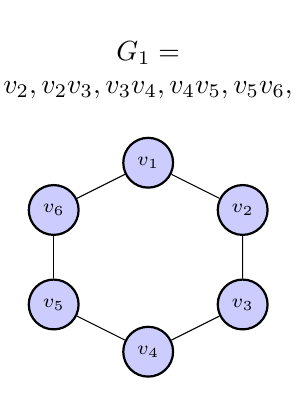
\begin{tikzpicture}
  [scale=.6, auto=left, 
   vertex/.style={circle, fill=blue!20, draw=black, thick, inner sep=2pt, minimum size=18pt}]

  \node[vertex] (n1) at (2,4) {$\scriptstyle v_1$};
  \node[vertex] (n2) at (4,3) {$\scriptstyle v_2$};
  \node[vertex] (n3) at (4,1) {$\scriptstyle v_3$};
  \node[vertex] (n4) at (2,0) {$\scriptstyle v_4$};
  \node[vertex] (n5) at (0,1) {$\scriptstyle v_5$};
  \node[vertex] (n6) at (0,3) {$\scriptstyle v_6$};

  \foreach \from/\to in {n1/n2,n2/n3,n3/n4,n4/n5,n5/n6,n6/n1}
    \draw (\from) -- (\to);

  \node[anchor=south, yshift=0.3cm] at (n1.north) {%
    \makebox[0pt][c]{%
      $\begin{array}{c}
        G_1=\\
        (V,\{v_1v_2,v_2v_3,v_3v_4,v_4v_5,v_5v_6, v_6v_1\})
      \end{array}$%
    }%
  };
\end{tikzpicture}
%
  }%
  \hfill
  \makebox[0.48\textwidth][c]{%
    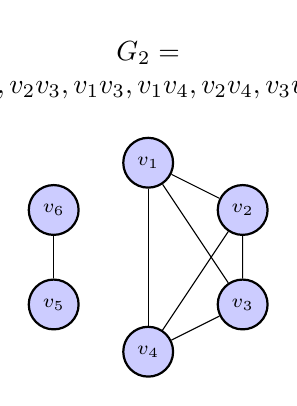
\begin{tikzpicture}
  [scale=.6, auto=left, 
   vertex/.style={circle, fill=blue!20, draw=black, thick, inner sep=2pt, minimum size=18pt}]

  \node[vertex] (n1) at (2,4) {$\scriptstyle v_1$};
  \node[vertex] (n2) at (4,3) {$\scriptstyle v_2$};
  \node[vertex] (n3) at (4,1) {$\scriptstyle v_3$};
  \node[vertex] (n4) at (2,0) {$\scriptstyle v_4$};
  \node[vertex] (n5) at (0,1) {$\scriptstyle v_5$};
  \node[vertex] (n6) at (0,3) {$\scriptstyle v_6$};

  \foreach \from/\to in {n1/n2,n2/n3,n1/n3, n1/n4, n2/n4, n3/n4,n5/n6}
    \draw (\from) -- (\to);

  \node[anchor=south, yshift=0.3cm] at (n1.north) {%
    \makebox[0pt][c]{%
      $\begin{array}{c}
        G_2=\\
        (V,\{v_1v_2, v_2v_3, v_1v_3, v_1v_4, v_2v_4, v_3v_4, v_5v_6\})
      \end{array}$%
    }%
  };
\end{tikzpicture}
%
  }\par

  \vspace{1.5em}% Separación vertical entre filas de diagramas

  % ================= FILA 2 =================
  \makebox[0.48\textwidth][c]{%
    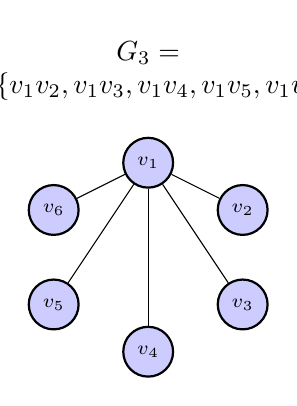
\begin{tikzpicture}
  [scale=.6, auto=left, 
   vertex/.style={circle, fill=blue!20, draw=black, thick, inner sep=2pt, minimum size=18pt}]

  \node[vertex] (n1) at (2,4) {$\scriptstyle v_1$};
  \node[vertex] (n2) at (4,3) {$\scriptstyle v_2$};
  \node[vertex] (n3) at (4,1) {$\scriptstyle v_3$};
  \node[vertex] (n4) at (2,0) {$\scriptstyle v_4$};
  \node[vertex] (n5) at (0,1) {$\scriptstyle v_5$};
  \node[vertex] (n6) at (0,3) {$\scriptstyle v_6$};

  \foreach \from/\to in {n1/n2, n1/n3, n1/n4, n1/n5, n1/n6}
    \draw (\from) -- (\to);

  \node[anchor=south, yshift=0.3cm] at (n1.north) {%
    \makebox[0pt][c]{%
      $\begin{array}{c}
        G_3=\\
        (V, \{v_1v_2, v_1v_3, v_1v_4, v_1v_5, v_1v_6\})
      \end{array}$%
    }%
  };
\end{tikzpicture}
%
  }%
  \hfill
  \makebox[0.48\textwidth][c]{%
    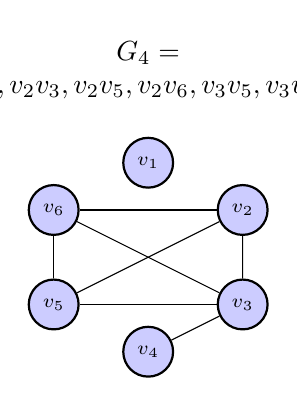
\begin{tikzpicture}
  [scale=.6, auto=left, 
   vertex/.style={circle, fill=blue!20, draw=black, thick, inner sep=2pt, minimum size=18pt}]

  \node[vertex] (n1) at (2,4) {$\scriptstyle v_1$};
  \node[vertex] (n2) at (4,3) {$\scriptstyle v_2$};
  \node[vertex] (n3) at (4,1) {$\scriptstyle v_3$};
  \node[vertex] (n4) at (2,0) {$\scriptstyle v_4$};
  \node[vertex] (n5) at (0,1) {$\scriptstyle v_5$};
  \node[vertex] (n6) at (0,3) {$\scriptstyle v_6$};

  \foreach \from/\to in {n3/n4,n2/n3, n2/n5, n2/n6, n3/n5, n3/n6, n5/n6}
    \draw (\from) -- (\to);

  \node[anchor=south, yshift=0.3cm] at (n1.north) {%
    \makebox[0pt][c]{%
      $\begin{array}{c}
        G_4=\\
        (V,\{v_3v_4, v_2v_3, v_2v_5, v_2v_6, v_3v_5, v_3v_6, v_5v_6\})
      \end{array}$%
    }%
  };
\end{tikzpicture}
%
  }\par

  \vspace{1.2em}% Espacio entre los diagramas y el título/caption
  \captionof{figure}{Ejemplos de grafos sobre $V$}
  \label{fig:ejemplos_grafos_conjuntos}
\par}
\phantom{o}\\

   Un ejemplo de grafo sobre $V'=\left\lbrace v_1, v_2, v_3, \dots\right\rbrace$ es $G_5=(V',\left\lbrace v_1v_2, v_2v_3, v_3v_4, v_4v_5, \dots\right\rbrace)$.
   \begin{figure}[H]
     \centering
       \resizebox{0.45\textwidth}{!}{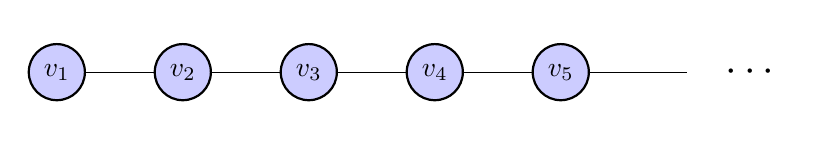
\begin{tikzpicture}
  [scale=.8,auto=left,every node/.style={circle,fill=blue!20,draw=black,thick}]
  \node (n1) at (0,0) {$v_1$};
  \node (n2) at (2,0)  {$v_2$};
  \node (n3) at (4,0)  {$v_3$};
  \node (n4) at (6,0) {$v_4$};
  \node (n5) at (8,0)  {$v_5$};

  \foreach \from/\to in {n1/n2,n2/n3, n3/n4, n4/n5}
    \draw (\from) -- (\to);

   %Flecha de (n5) a un nodo invisible en (10,0)   
   \draw (n5) -- (10,0);
   
   %Etiqueta de puntos suspensivos
   \node[draw=none, fill=none, scale=1.5] at (11,0) {$\cdots$};
   % Etiqueta G_1 debajo del grafo
%   \node[draw=none, fill=none, scale=1.5] at (6,-1.5) {$G_5$};
\end{tikzpicture}
} 
     \caption{El grafo $G_5$ sobre $V'$}
   \end{figure}
\end{Ejm}
\begin{Not}
   El grafo $G=(\emptyset,\emptyset)$ en el cual tanto el conjunto de vértices como el de aristas son vacíos, lo llamamos \textbf{grafo vacío} y lo representamos simplemente por $\emptyset$.
\end{Not}
Notemos que en un grafo $G$, dada $uv\in E(G)$, se tiene que $uv$ y $vu$ hacen referencia a la misma arista, pues $uv=\left\lbrace u,v \right\rbrace=\left\lbrace v, u\right\rbrace=vu$. De esta forma, en un grafo, el orden de los vértices en la representación de una arista no es tenido en cuenta, lo cual está alineado con nuestra idea de no considerar orientación en ella. Además, la exigencia de que las aristas de un grafo sean $2-subconjuntos$ de vértices implica que si $uv\in E(G)$ entonces $u\neq v$, es decir, no hay aristas que unan un vértice con sí mismo, de modo que los grafos que consideramos no tienen bucles. Así mismo, entre dos vértices distintos $u,v\in V(G)$ podrá haber a lo más una arista, dependiendo de si $uv$ pertenece a $E(G)$ o no, es decir, se excluye la posibilidad de que hayan aristas múltiples entre un par de vértices.\par
Frecuentemente en matemáticas, uno de los primeros pasos al analizar una estructura formal es estudiar sus subestructuras, es decir, objetos del mismo tipo contenidos en ella. Para esto introducimos la noción de \textit{subgrafo}.\clearpage
\begin{Def}
   Dados dos grafos $G=(V,E)$ y $G'=(V',E')$, decimos que $G'$ es un \textbf{subgrafo} de $G$ si $V'\subseteq V$ y $E'\subseteq E$. En este caso denotamos $G'\subseteq G$.
\end{Def}
Para cualquier grafo $G$ se tiene $\emptyset\subseteq G$. Damos a continuación más ejemplos de contenencia de grafos.
\begin{Ejm}\label{Ejm:Contenencia}
   En cada fila de la \Cref{tab:grafos} se tiene $G'\subseteq G$.
   \par\vspace{1em}
\begin{longtable}{|c|c|c|}
  \hline
  \rule[-0.5em]{0pt}{1.8em} & \rule[-0.5em]{0pt}{1.8em} $G$ & \rule[-0.5em]{0pt}{1.8em} $G'$ \\
  \hline
  \endhead
  \hline
  \endfoot
  \caption{Ejemplos de contenencia de grafos} \addtocounter{table}{-1}\refstepcounter{table}\label{tab:grafos} \\
  \endlastfoot

  $G_1 \subseteq G'_1$ &
  \begin{minipage}{0.3\textwidth} \centering \vspace{8pt} \resizebox{0.85\linewidth}{!}{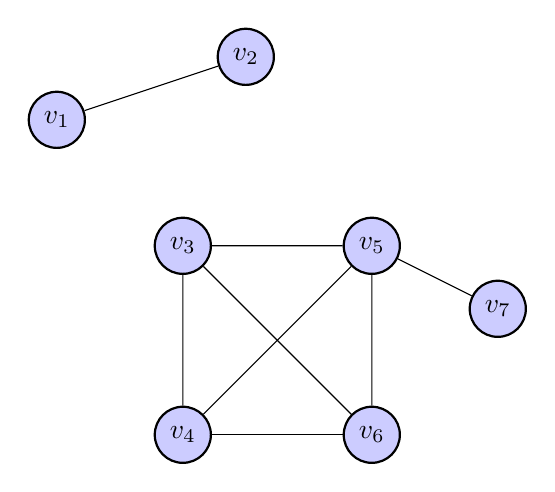
\begin{tikzpicture}
   [scale=.8,auto=left,every node/.style={circle,fill=blue!20,draw=black,thick}]
  \node (n1) at (0,5) {$v_1$};
  \node (n2) at (3,6) {$v_2$};
  \node (n3) at (2,3) {$v_3$};
  \node (n4) at (2,0) {$v_4$};
  \node (n5) at (5,3) {$v_5$};
  \node (n6) at (5,0) {$v_6$};
  \node (n7) at (7,2) {$v_7$};

  \foreach \from/\to in {n1/n2, n3/n5, n5/n6, n6/n4, n4/n3, n3/n6, n4/n5, n5/n7}
    \draw (\from) -- (\to);

\end{tikzpicture}
} \vspace{6pt} \end{minipage} &
  \begin{minipage}{0.3\textwidth} \centering \vspace{8pt} \resizebox{0.85\linewidth}{!}{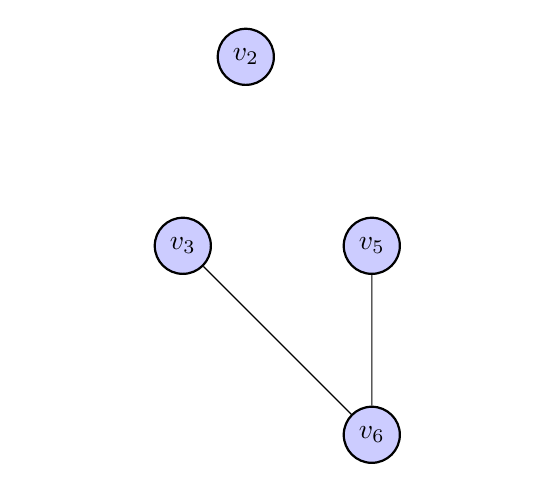
\begin{tikzpicture}
  [scale=.8,auto=left,every node/.style={circle,fill=blue!20,draw=black,thick}]
  \node (n1) at (0,5) [opacity=0] {$v_1$};
  \node (n2) at (3,6) {$v_2$};
  \node (n3) at (2,3) {$v_3$};
  \node (n4) at (2,0) [opacity=0]{$v_4$};
  \node (n5) at (5,3) {$v_5$};
  \node (n6) at (5,0) {$v_6$};
  \node (n7) at (7,2) [opacity=0]{$v_7$};

  \foreach \from/\to in {n1/n2, n3/n5, n5/n6, n6/n4, n4/n3, n3/n6, n4/n5, n5/n7}
    \draw[opacity=0] (\from) -- (\to);
   
    \foreach \from/\to in {n3/n6, n5/n6}
     \draw[opacity=1] (\from) -- (\to);

  \end{tikzpicture}
} \vspace{6pt} \end{minipage} \\
  \hline

  $G_2 \subseteq G'_2$ &
  \begin{minipage}{0.3\textwidth} \centering \vspace{8pt} \resizebox{0.8\linewidth}{!}{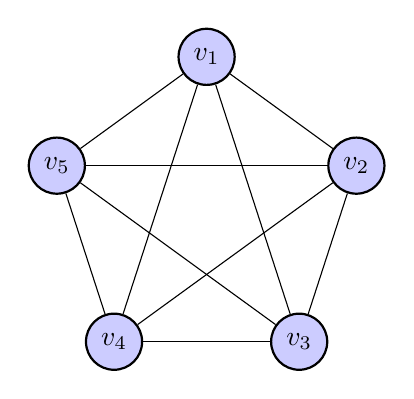
\begin{tikzpicture}
  [scale=1,auto=left,every node/.style={circle,fill=blue!20,draw=black,thick}]
  \node (n1) at (90:2) {$v_1$};
  \node (n2) at (18:2) {$v_2$};
  \node (n3) at (-54:2) {$v_3$};
  \node (n4) at (-126:2) {$v_4$};
  \node (n5) at (-198:2) {$v_5$};

  \foreach \from/\to in {n1/n2, n1/n3, n1/n4, n1/n5, n2/n3, n2/n4, n2/n5, n3/n4, n3/n5, n4/n5}
    \draw (\from) -- (\to);

 \end{tikzpicture}
} \vspace{6pt} \end{minipage} &
  \begin{minipage}{0.3\textwidth} \centering \vspace{8pt} \resizebox{0.8\linewidth}{!}{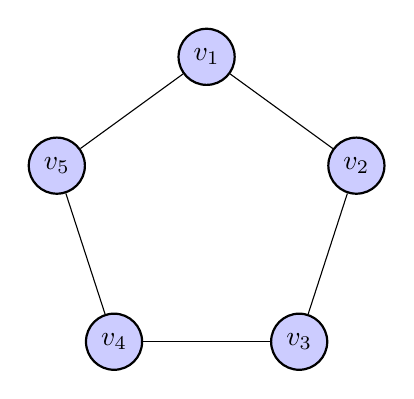
\begin{tikzpicture}
  [scale=1,auto=left,every node/.style={circle,fill=blue!20,draw=black,thick}]
  \node (n1) at (90:2) {$v_1$};
  \node (n2) at (18:2) {$v_2$};
  \node (n3) at (-54:2) {$v_3$};
  \node (n4) at (-126:2) {$v_4$};
  \node (n5) at (-198:2) {$v_5$};

  \foreach \from/\to in {n1/n2, n2/n3, n3/n4, n4/n5, n5/n1}
    \draw (\from) -- (\to);

 \end{tikzpicture}
} \vspace{6pt} \end{minipage} \\
  \hline

  $G_3 \subseteq G'_3$ &
  \begin{minipage}{0.3\textwidth} \centering \vspace{8pt} \resizebox{0.8\linewidth}{!}{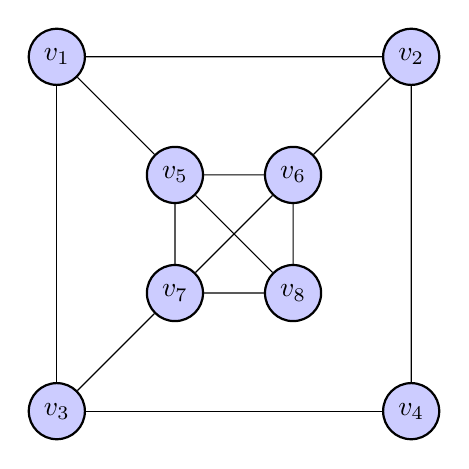
\begin{tikzpicture}
  [scale=1.5,auto=left,every node/.style={circle,fill=blue!20,draw=black,thick}]
  \node (n1) at (0,3) {$v_1$};
  \node (n2) at (3,3) {$v_2$};
  \node (n3) at (0,0) {$v_3$};
  \node (n4) at (3,0) {$v_4$};
  \node (n5) at (1,2) {$v_5$};
  \node (n6) at (2,2) {$v_6$};
  \node (n7) at (1,1) {$v_7$};
  \node (n8) at (2,1) {$v_8$};

  \foreach \from/\to in {n1/n2, n1/n3, n2/n4, n3/n7, n6/n7, n1/n5, n2/n6, n5/n6, n6/n8, n7/n8, n7/n5, n5/n8, n3/n4}
    \draw (\from) -- (\to);

 \end{tikzpicture}
} \vspace{6pt} \end{minipage} &
  \begin{minipage}{0.3\textwidth} \centering \vspace{8pt} \resizebox{0.8\linewidth}{!}{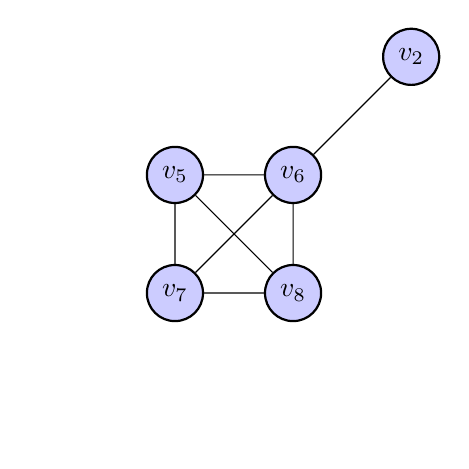
\begin{tikzpicture}
  [scale=1.5,auto=left,every node/.style={circle,fill=blue!20,draw=black,thick}]
  \node (n1) at (0,3) [opacity=0] {$v_1$};
  \node (n2) at (3,3) {$v_2$};
  \node (n3) at (0,0) [opacity=0] {$v_3$};
  \node (n4) at (3,0) [opacity=0] {$v_4$};
  \node (n5) at (1,2) {$v_5$};
  \node (n6) at (2,2) {$v_6$};
  \node (n7) at (1,1) {$v_7$};
  \node (n8) at (2,1) {$v_8$};

  \foreach \from/\to in {n2/n6, n5/n6, n6/n8, n7/n8, n7/n5, n5/n8, n6/n7}
    \draw (\from) -- (\to);

 \end{tikzpicture}
} \vspace{6pt} \end{minipage} \\
  \hline
\end{longtable}
\par\vspace{-0.3em}

\end{Ejm}\clearpage
En el \Cref{Ejm:Contenencia} se cumple que $G'_3$ conserva todas las aristas entre vértices de $V(G'_3)$ que aparecían originalmente en $G_3$, es decir, para cualesquiera $u,v\in V(G'_3)$ se tiene que $uv\in E(G_3)$ implica $uv\in E(G'_3)$. Notemos que en los ejemplos $G_1$ y $G_2$ esto no se cumple. Por ejemplo, para $G_1$ se tiene $v_3,v_5\in V(G'_1)$ y $v_3v_5\in E(G_1)$, pero $v_3v_5 \notin E(G'_1)$; para $G_2$ se tiene $v_1,v_3\in V(G'_2)$ y $v_1v_3\in E(G_2)$, pero $v_1v_3\notin E(G'_2)$. El comportamiento que se da con $G_3$ y $G'_3$ lo resumimos diciendo que $G'_3$ es el \textit{subgrafo de $G_3$ inducido} por $V(G'_3)$, y denotamos $G'_3=G[V(G'_3)]$. Más precisamente:
\begin{Def}
   Sean $G$ un grafo y $W\subseteq V(G)$. El \textbf{subgrafo de $G$ inducido} por $W$, denotado por $G[W]$, se define como el subgrafo de $G$ tal que $V(G[W])=W$ y $E(G[W])=\left\lbrace uv\in E(G)\mid u,v\in W\right\rbrace$.
\end{Def}
\begin{Ejm}
   \phantom{o}
   \begin{itemize}
      \item $G_2$ es el subgrafo de $G_1$ inducido por $W=\left\lbrace v_2,v_3,v_4,v_5,v_6\right\rbrace$:
         \begin{figure}[H]
  \centering
  \resizebox{0.2\textwidth}{!}{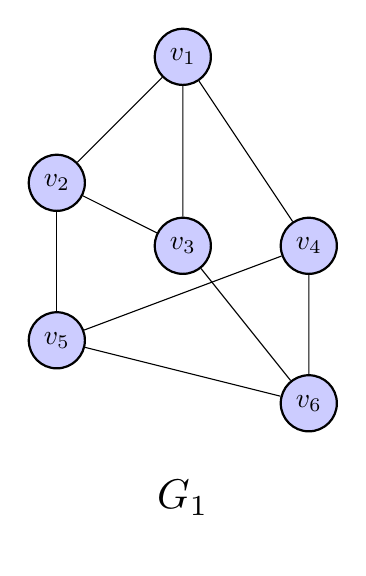
\begin{tikzpicture}
  [scale=.8,auto=left,every node/.style={circle,fill=blue!20,draw=black,thick}]
  \node (n1) at (3,6) {$v_1$};
  \node (n2) at (1,4) {$v_2$};
  \node (n3) at (3,3) {$v_3$};
  \node (n4) at (5,3) {$v_4$};
  \node (n5) at (1,1.5) {$v_5$};
  \node (n6) at (5,0.5) {$v_6$};

  \foreach \from/\to in {n1/n2, n1/n3, n1/n4, n2/n3, n2/n5, n3/n6, n4/n5, n4/n6, n5/n6}
    \draw (\from) -- (\to);

   \node[draw=none, fill=none, scale=1.5] at (3,-1) {$G_1$};
\end{tikzpicture}
} \hspace{2cm}
    \resizebox{0.2\textwidth}{!}{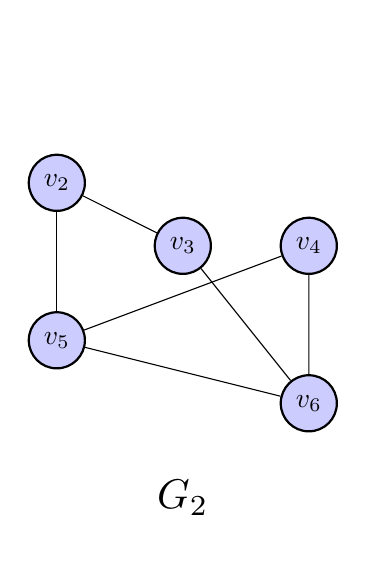
\begin{tikzpicture}
  [scale=.8,auto=left,every node/.style={circle,fill=blue!20,draw=black,thick}]
  \node (n1) at (3,6) [opacity=0] {$v_1$};
  \node (n2) at (1,4) {$v_2$};
  \node (n3) at (3,3) {$v_3$};
  \node (n4) at (5,3) {$v_4$};
  \node (n5) at (1,1.5) {$v_5$};
  \node (n6) at (5,0.5) {$v_6$};

  \foreach \from/\to in {n2/n3, n2/n5, n3/n6, n4/n5, n4/n6, n5/n6}
    \draw (\from) -- (\to);


   \node[draw=none, fill=none, scale=1.5] at (3,-1) {$G_2$};
\end{tikzpicture}
} 
    \caption{$G_2=G_1[W]$}
\end{figure}
  
      \item $G_4$ es el subgrafo de $G_3$ inducido por $W'=\left\lbrace v_1,v_2,v_3,v_5\right\rbrace$:
         \vspace{-4em}
\begin{figure}[H]
  \hspace*{3.9cm}%
  \resizebox{0.23\textwidth}{!}{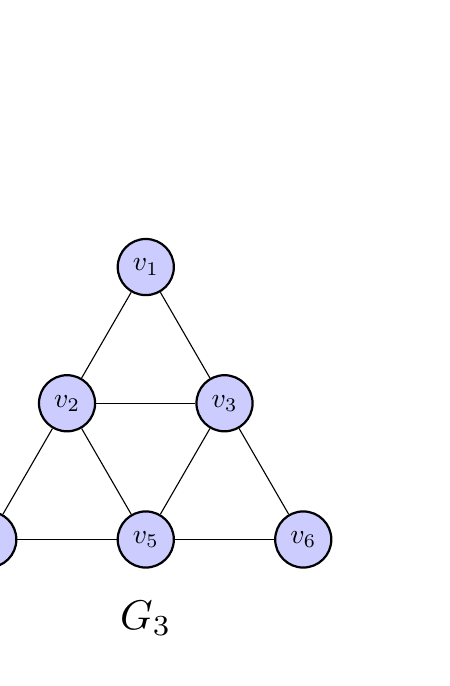
\begin{tikzpicture}
  [scale=1,auto=left,every node/.style={circle,fill=blue!20,draw=black,thick}]
\useasboundingbox (0.5,-1.5) rectangle (5.5,6.5);
  % Posiciones simétricas en forma de triángulo equilátero
  \node (n1) at (2,3.46) {$v_1$};
  \node (n2) at (1,1.73) {$v_2$};
  \node (n3) at (3,1.73) {$v_3$};
  \node (n4) at (0,0)    {$v_4$};
  \node (n5) at (2,0)    {$v_5$};
  \node (n6) at (4,0)    {$v_6$};

  % Aristas del grafo base (malla triangular)
  \foreach \from/\to in {n1/n2, n1/n3, n2/n3, n2/n4, n2/n5, n3/n5, n3/n6, n4/n5, n5/n6}
    \draw (\from) -- (\to);

   \node[draw=none, fill=none, scale=1.5] at (2,-1) {$G_3$};
\end{tikzpicture}
}
  \hspace*{1.15cm}
    \resizebox{0.23\textwidth}{!}{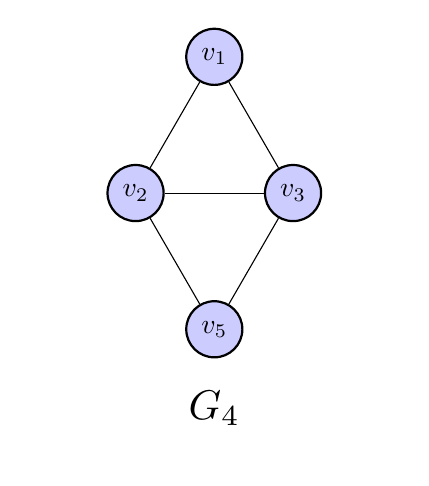
\begin{tikzpicture}
  [scale=1,auto=left,every node/.style={circle,fill=blue!20,draw=black,thick}]
  % Posiciones simétricas en forma de triángulo equilátero
  \node (n1) at (2,3.46) {$v_1$};
  \node (n2) at (1,1.73) {$v_2$};
  \node (n3) at (3,1.73) {$v_3$};
  \node (n4) at (0,0)   [opacity=0] {$v_4$};
  \node (n5) at (2,0)    {$v_5$};
  \node (n6) at (4,0)   [opacity=0] {$v_6$};

  % Aristas del grafo base (malla triangular)
  \foreach \from/\to in {n1/n2, n1/n3, n2/n3, n2/n5, n3/n5}
    \draw (\from) -- (\to);

   \node[draw=none, fill=none, scale=1.5] at (2,-1) {$G_4$};
\end{tikzpicture}
} 
    \caption{$G_4=G_3[W']$}
\end{figure}
  
   \end{itemize}
\end{Ejm}
\begin{Def}
   El \textbf{orden} de un grafo $G$, representado mediante $|G|$, es el cardinal del conjunto $V(G)$.
\end{Def}
Así, en el \Cref{Ejm:cuatro_grafos}, el grado de los cuatro primeros grafos es $6$, mientras que $|G_5|=\aleph _0$. Los grafos pueden ser \textit{finitos, infinitos, contables}, etc., dependiendo del respectivo tamaño del conjunto $G$.
\begin{Def}
   Dado un grafo $G$, decimos que dos vértices $u,v\in V(G)$ son \textbf{adyacentes} si $uv\in E(G)$. Igualmente, decimos que el vértice $v\in V(G)$ es \textbf{incidente} con la arista $e\in E(G)$ si $v\in e$. 
\end{Def}
En el grafo $G_1$ del \Cref{Ejm:cuatro_grafos}, los vértices $v_3$ y $v_4$ son adyacentes, los vértices $v_2$ y $v_5$ no son adyacentes, el vértice $v_6$ es incidente con la arista $v_1v_6$ y el vértice $v_4$ no es incidente con la arista $v_2v_3$. Los grafos finitos permiten una representación mediante matrices basada en las relaciones de adyacencia de sus vértices.
\begin{Def}
   Sea $G$ un grafo con $V(G)=\left\lbrace v_1,\dots ,v_n\right\rbrace$ para algún $n\in\mathbb{Z}^+$. La \textbf{matriz de adyacencia} $A=(a_{ij})_{n\times n}$ de $G$ se define mediante
   $$
   a_{ij} := \begin{cases} 
     1 & \text{si } v_iv_j \in E(G) \\ 
     0 & \text{en otro caso.} 
   \end{cases}
   $$
   Si $G=\emptyset$, definimos la matriz de adyacencia de $G$ como la matriz vacía de tamaño $0\times 0$.
\end{Def}
El uso de matrices de adyacencia para la representación de grafos finitos presenta utilidades para su manejo mediante computadoras. Como afirma \cite{marimont1960}, aunque los grafos representados visualmente son ``intuitivamente sugestivos y fáciles de comprender'', su manejo directo mediante computadoras resulta inviable, no se presta a manipulaciones cuantitativas inmediatas, y a medida que crecen en tamaño y complejidad, se va perdiendo la intuición que en principio proporcionan. Las matrices en cambio, pueden ser manipuladas fácilmente por computadoras, las cuales sacan vasto provecho del procesamiento cuantitativo que ofrecen, a pesar del poco atractivo intuitivo que pueda presentar al ojo humano frente a la representación visual del grafo. En las \Cref{sec:computacional_adyacencia,sec:computacional_incidencia} hacemos uso de matrices de adyacencia en algunas implementaciones computacionales.\clearpage
\begin{Ejm}
   En cada fila de la \Cref{tab:grafos_matrices} se muestra un grafo finito $G$ y su respectiva matriz de adyacencia $M$.
   \par\vspace{1em}
\begin{longtable}{|c|c|c|}
  \hline
  \rule[-0.5em]{0pt}{1.8em} & \rule[-0.5em]{0pt}{1.8em} $G$ & \rule[-0.5em]{0pt}{1.8em} $M$ \\
  \hline
  \endhead
  \hline
  \endfoot
  \caption{Grafos y sus matrices de adyacencia} \addtocounter{table}{-1}\refstepcounter{table}\label{tab:grafos_matrices} \\
  \endlastfoot

  $G_1$ y $M_1$ &
  \begin{minipage}{0.3\textwidth} \centering \vspace{8pt} \resizebox{0.85\linewidth}{!}{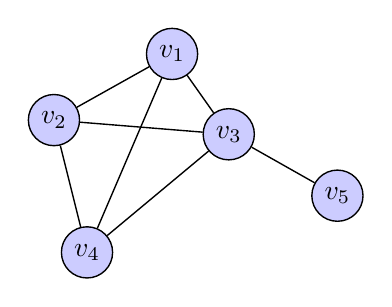
\begin{tikzpicture}[
  scale=0.6,
  vnode/.style={circle, fill=blue!20, draw=black, line width=0.5pt, inner sep=2pt, minimum size=6.5mm},
  edge/.style={line width=0.5pt, draw=black}
]

  % Posicionamiento de vértices asimétrico
  \node[vnode] (v1) at (0, 3.2) {$v_1$};
  \node[vnode] (v2) at (-2.5, 1.8) {$v_2$};
  \node[vnode] (v3) at (1.2, 1.5) {$v_3$};
  \node[vnode] (v4) at (-1.8, -1.0) {$v_4$};
  \node[vnode] (v5) at (3.5, 0.2) {$v_5$};

  % Aristas
  \draw[edge] (v1) -- (v2);
  \draw[edge] (v1) -- (v3);
  \draw[edge] (v2) -- (v4);
  \draw[edge] (v3) -- (v4);
  \draw[edge] (v3) -- (v5);
  \draw[edge] (v2) -- (v3);
  \draw[edge] (v1) -- (v4);

\end{tikzpicture}
} \vspace{6pt} \end{minipage} &
  \begin{minipage}{0.3\textwidth} \centering \vspace{8pt}
    $\begin{pmatrix}
      0 & 1 & 1 & 1 & 0 \\
      1 & 0 & 1 & 1 & 0 \\
      1 & 1 & 0 & 1 & 1 \\
      1 & 1 & 1 & 0 & 0 \\
      0 & 0 & 1 & 0 & 0
    \end{pmatrix}$
  \vspace{6pt} \end{minipage} \\
  \hline

  $G_2$ y $M_2$ &
  \begin{minipage}{0.3\textwidth} \centering \vspace{8pt} \resizebox{0.85\linewidth}{!}{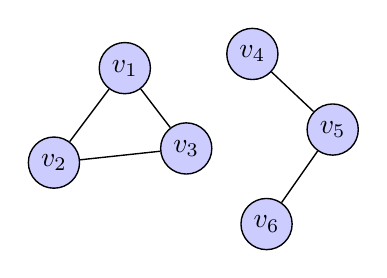
\begin{tikzpicture}[
  scale=0.6,
  vnode/.style={circle, fill=blue!20, draw=black, line width=0.5pt, inner sep=2pt, minimum size=6.5mm},
  edge/.style={line width=0.5pt, draw=black}
]

  % --- Componente 1 (Triángulo) ---
  \node[vnode] (v1) at (-2.5, 2.5) {$v_1$};
  \node[vnode] (v2) at (-4.0, 0.5) {$v_2$};
  \node[vnode] (v3) at (-1.2, 0.8) {$v_3$};

  \draw[edge] (v1) -- (v2) -- (v3) -- (v1);

  % --- Componente 2 (Camino/Trayectoria) ---
  \node[vnode] (v4) at (0.2, 2.8) {$v_4$};
  \node[vnode] (v5) at (1.9, 1.2) {$v_5$};
  \node[vnode] (v6) at (0.5, -0.8) {$v_6$};

  \draw[edge] (v4) -- (v5);
  \draw[edge] (v5) -- (v6);

\end{tikzpicture}
} \vspace{6pt} \end{minipage} &
  \begin{minipage}{0.3\textwidth} \centering \vspace{8pt}
    $\begin{pmatrix}
      0 & 1 & 1 & 0 & 0 & 0 \\
      1 & 0 & 1 & 0 & 0 & 0 \\
      1 & 1 & 0 & 0 & 0 & 0 \\
      0 & 0 & 0 & 0 & 1 & 0 \\
      0 & 0 & 0 & 1 & 0 & 1 \\
      0 & 0 & 0 & 0 & 1 & 0
    \end{pmatrix}$
  \vspace{6pt} \end{minipage} \\
  \hline

  $G_3$ y $M_3$ &
  \begin{minipage}{0.3\textwidth} \centering \vspace{8pt} \resizebox{0.85\linewidth}{!}{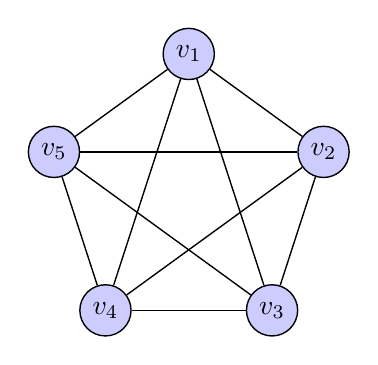
\begin{tikzpicture}[
  scale=1.0,
  vnode/.style={circle, fill=blue!20, draw=black, line width=0.5pt, inner sep=2pt, minimum size=6.5mm},
  edge/.style={line width=0.5pt, draw=black}
]

  % Vértices dispuestos en pentágono regular para máxima simetría
  \node[vnode] (v1) at (90:1.8) {$v_1$};
  \node[vnode] (v2) at (162:1.8) {$v_5$};
  \node[vnode] (v3) at (234:1.8) {$v_4$};
  \node[vnode] (v4) at (306:1.8) {$v_3$};
  \node[vnode] (v5) at (18:1.8) {$v_2$};

  % Todas las conexiones de un grafo completo K5 (10 aristas)
  \draw[edge] (v1) -- (v2);
  \draw[edge] (v1) -- (v3);
  \draw[edge] (v1) -- (v4);
  \draw[edge] (v1) -- (v5);

  \draw[edge] (v2) -- (v3);
  \draw[edge] (v2) -- (v4);
  \draw[edge] (v2) -- (v5);

  \draw[edge] (v3) -- (v4);
  \draw[edge] (v3) -- (v5);

  \draw[edge] (v4) -- (v5);

\end{tikzpicture}
} \vspace{6pt} \end{minipage} &
  \begin{minipage}{0.3\textwidth} \centering \vspace{8pt}
    $\begin{pmatrix}
      0 & 1 & 1 & 1 & 1 \\
      1 & 0 & 1 & 1 & 1 \\
      1 & 1 & 0 & 1 & 1 \\
      1 & 1 & 1 & 0 & 1 \\
      1 & 1 & 1 & 1 & 0
    \end{pmatrix}$
  \vspace{6pt} \end{minipage} \\
  \hline
\end{longtable}
\par\vspace{-0.3em}

\end{Ejm}
La ausencia de bucles en los grafos hace que todas las entradas en la diagonal principal de una matriz de adyacencia sean siempre $0$. Igualmente, el hecho de que en un grafo $G$ se tenga $v_iv_j\in E(G)$ si y sólo si $v_jv_i\in E(G)$, hace que cualquier matriz de adyacencia sea simétrica.\clearpage
\begin{Def}
   Sea $G$ un grafo. Dado un vértice $v\in V(G)$, denotamos por $\bm{A_v}$ al conjunto de todos los vértices adyacentes a $v$, es decir $A_v=\left\lbrace u\in V(G) \mid uv\in E(G)\right\rbrace$, y por $\bm{E_v}$ al conjunto de todas las aristas con las cuales es incidente $v$, es decir $E_v=\left\lbrace e\in E(G)\mid v\in e\right\rbrace$.
\end{Def}
De nuestra definicón de grafo se sigue inmediatamente que para cualquier par de vértices $u,v$ de un grafo, $u\in A_v$ si, y solo si, $v\in A_u$. En el grafo $G_2$ del \Cref{Ejm:cuatro_grafos}, tenemos que $A_{v_1}=\lbrace v_2,v_3,v_4\rbrace$, $A_{v_6}=\lbrace v_5\rbrace$, $E_{v_1}=\lbrace v_1v_2,v_1v_3,v_1v_4 \rbrace$ y $E_{v_6}=\lbrace v_5v_6\rbrace$. En el grafo $G_5$ del mismo ejemplo se tiene, para todo $i\in \left\lbrace 2,3,4,\dots\right\rbrace$, $A_{v_i}=\left\lbrace v_{i-1}, v_{i+1}\right\rbrace$ y $E_{v_i}=\left\lbrace v_{i-1}v_i, v_iv_{i+1}\right\rbrace$.\\
La siguiente proposición nos muestra el hecho natural de que la cantidad de vértices adyacentes a $v$ y la cantidad de aristas con las cuales es incidente $v$ es siempre la misma para, cualquier vértice $v$ en un grafo arbitrario.
\begin{Prop} \label{Prop:AvEv}
   En cualquier grafo $G$, dado $v\in V(G)$, se tiene $|A_v|=|E_v|$.
\end{Prop}
\begin{proof}
Definamos $f:A_v\to E_v: u\mapsto uv$. Nótese que si $u\in A_v$, entonces $uv\in E(G)$, y $v\in uv$, luego $uv\in E_v$, de modo que $f$ está bien definida. Se tiene que $f$ es inyectiva, pues si $u_1,u_2 \in A_v$ son tales que $f(u_1)=f(u_2)$ entonces $u_1v=u_2v$, es decir $\left\lbrace u_1,v\right\rbrace=\left\lbrace u_2,v\right\rbrace$, y como $u_1\neq v$ y $u_2\neq v$, entonces $u_1=u_2$. Además $f$ es sobreyectiva, pues dada $e\in E_v$, tenemos $v\in e$ y por tanto $e=uv$ para algún $u\in V(G)$; en particular $uv\in E(G)$, luego $u\in A_v$, y $f(u)=uv=e$. Por tanto $f$ es una biyección, con lo cual $|A_v|=|E_v|$.
\end{proof}
\begin{Def}
   Sea $G$ un grafo. El \textbf{grado} de un vértice $v\in V(G)$ se define como $d(v):=|A_v|$. Un vértice de grado $0$ se llama \textbf{aislado}, y uno de grado $1$ se llama una \textbf{hoja}.
\end{Def}
De este modo, el grado de un vértice se define como la cantidad de vértices adyacentes con él, que por la \Cref{Prop:AvEv}, es igual a la cantidad de aristas con las cuales es incidente. En el grafo $G_4$ del \Cref{Ejm:cuatro_grafos} se tiene $d(v_2)=3$ y $d(v_3)=4$, mientras que $v_1$ es un vértice aislado y $v_4$ es una hoja. En el grafo $G_5$ del mismo ejemplo se tiene $d(v_1)=1$ y $d(v_i)=2$ para todo $i\in \left\lbrace 2,3,4,\dots \right\rbrace$.
\begin{Def}
   Sea $G$ un grafo. Definimos el \textbf{grado mínimo} de $G$ como $\delta (G):= \min \left\lbrace d(v)\mid v\in V\right\rbrace$ y el \textbf{grado máximo} de $G$ como $\Delta (G):= \max \left\lbrace d(v)\mid v\in V\right\rbrace$, siempre que estos valores estén bien definidos.
\end{Def}
En el \Cref{Ejm:cuatro_grafos}, $\delta (G_1)=2=\Delta (G_1)$, $\delta (G_2)=1$, $\Delta (G_2)=3$, $\delta (G_3)=1$, $\Delta (G_3)=5$, $\delta (G_4)=0$, $\Delta (G_4)=4$, $\delta (G_5)=1$, $\Delta (G_5)=2$.
\begin{Def}
   Un grafo en el cual todos los vértices tienen el mismo grado $k$ se dice $\boldsymbol{k}$\textbf{-regular}, o simplemente \textbf{regular}.
\end{Def}
El grafo $G_1$ del \Cref{Ejm:cuatro_grafos} es $2$-regular. Naturalmente, en cualquier grafo $k$-regular $G$ se tiene $\delta(G)=\Delta(G)=k$.
\begin{Def}
   Un grafo se dice \textbf{localmente finito} si todos sus vértices tienen grado finito. 
\end{Def}
Todos los grafos finitos son localmente finitos. El grafo $G_5$ del \Cref{Ejm:cuatro_grafos} es un ejemplo de grafo infinito localmente finito. Se tienen otras situaciones, como se muestra a continuación.
\begin{Ejm}
   \phantom{o}
   \begin{figure}[H]
     \centering
       \resizebox{0.4\textwidth}{!}{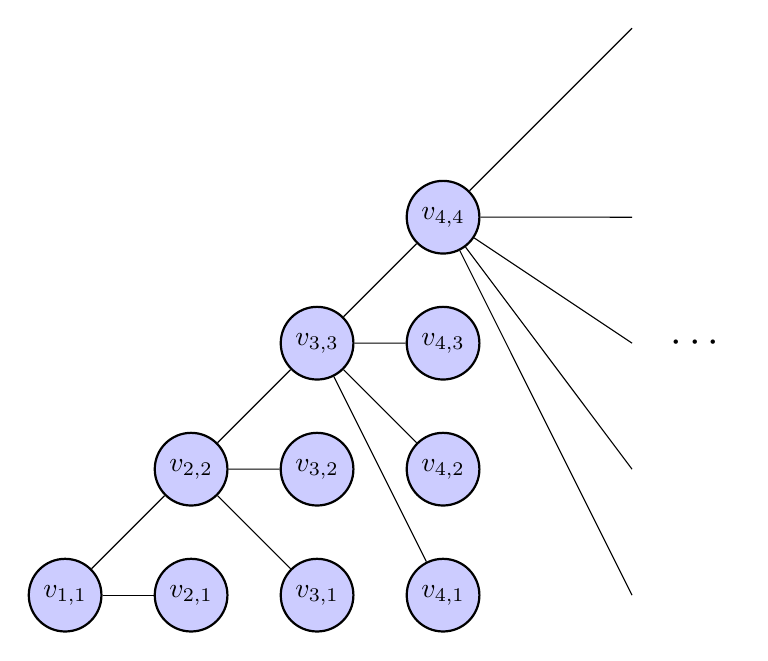
\begin{tikzpicture}
  [scale=.8,auto=left,every node/.style={circle,fill=blue!20,draw=black,thick}]
  \node (n1) at (0,0) {$v_{1,1}$};
  \node (n2) at (2,0)  {$v_{2,1}$};
  \node (n3) at (2,2)  {$v_{2,2}$};
  \node (n4) at (4,0) {$v_{3,1}$};
  \node (n5) at (4,2)  {$v_{3,2}$};
  \node (n6) at (4,4)  {$v_{3,3}$};
  \node (n7) at (6,0)  {$v_{4,1}$};
  \node (n8) at (6,2)  {$v_{4,2}$};
  \node (n9) at (6,4)  {$v_{4,3}$};
  \node (n10) at (6,6)  {$v_{4,4}$};

  \foreach \from/\to in {n1/n2,n1/n3, n3/n4, n3/n5, n3/n6, n6/n7, n6/n8, n6/n9, n6/n10}
    \draw (\from) -- (\to);

   \draw (n10) -- (9,0);
   \draw (n10) -- (9,2);
   \draw (n10) -- (9,4);
   \draw (n10) -- (9,6);
   \draw (n10) -- (9,9);
   
   %Etiqueta de puntos suspensivos
   \node[draw=none, fill=none, scale=1.5] at (10,4) {$\cdots$};
\end{tikzpicture}
} 
     \caption{Un grafo infinito localmente finito}
   \end{figure}
\end{Ejm}
\begin{Ejm}
   El siguiente grafo infinito no es localmente finito, pues $d(v_1)$ no es finito.
   \begin{figure}[H]
     \centering
       \resizebox{0.45\textwidth}{!}{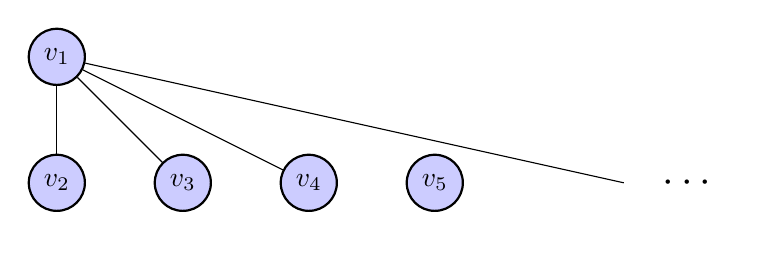
\begin{tikzpicture}
  [scale=.8,auto=left,every node/.style={circle,fill=blue!20,draw=black,thick}]
  \node (n1) at (0,2)  {$v_1$};
  \node (n2) at (0,0)  {$v_2$};
  \node (n3) at (2,0)  {$v_3$};
  \node (n4) at (4,0)  {$v_4$};
  \node (n5) at (6,0)  {$v_5$};


   \foreach \from/\to in {n1/n2,n1/n3, n1/n4}
      \draw (\from) -- (\to);
   
   \draw (n1) -- (9,0);

   \node[draw=none, fill=none, scale=1.5] at (10,0) {$\cdots$};
   
\end{tikzpicture}

} 
     \caption{Un grafo infinito que no es localmente finito}
   \end{figure}
\end{Ejm}
Un concepto importante en el presente trabajo es el de \textit{grafo conexo}. Para ello introducimos primero la definición de \textit{camino}.
\begin{Def}
   Un \textbf{camino} es un grafo no vacío $P=(V,E)$ de la forma
   $$
   V=\left\lbrace x_0, x_1, \dots, x_k\right\rbrace, \quad E=\left\lbrace x_0x_1, x_1x_2, \dots , x_{k-1}x_k\right\rbrace,
   $$
   para $k\in \mathbb{N}$, y donde todos los $x_i$, con $i\in \left\lbrace 0,1,\dots,k\right\rbrace$, son distintos. En este caso denotamos a $P$ mediante $x_0x_1\dots x_k$ o $x_kx_{k-1}\dots x_0$. Decimos que los vértices $x_0$ y $x_k$ están \textbf{conectados} por el camino P, y que $x_0$ y $x_k$ son los \textbf{extremos} de $P$. El número de aristas de un camino es su \textbf{longitud}. Denotamos por $\bm{P^k}$ a cualquier camino con $k$ vértices.
\end{Def}
\begin{Ejm}
   \phantom{o}
   \begin{itemize}
      \item $P^1$ es el grafo conformado por un solo vértice; es un camino de longitud $0$.
      \item Un camino de longitud $6$ es el siguiente:
      \begin{figure}[H]
        \centering
          \resizebox{0.3\textwidth}{!}{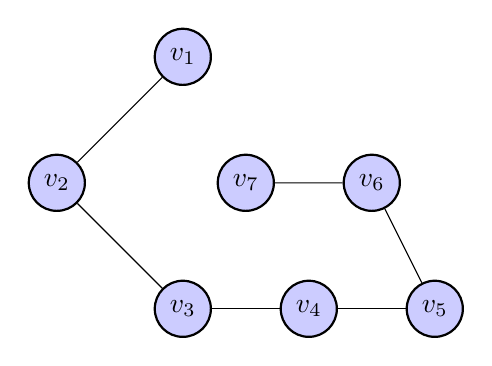
\begin{tikzpicture}
  [scale=.8,auto=left,every node/.style={circle,fill=blue!20,draw=black,thick}]
  \node (n1) at (2,4) {$v_1$};
  \node (n2) at (0,2)  {$v_2$};
  \node (n3) at (2,0)  {$v_3$};
  \node (n4) at (4,0) {$v_4$};
  \node (n5) at (6,0)  {$v_5$};
  \node (n6) at (5,2)  {$v_6$};
  \node (n7) at (3,2)  {$v_7$};

  \foreach \from/\to in {n1/n2,n2/n3, n3/n4, n4/n5, n5/n6, n6/n7}
    \draw (\from) -- (\to);
\end{tikzpicture}
}
        \caption{$P^7=v_1v_2v_3v_4v_5v_6v_7$}
      \end{figure}
   \end{itemize}
\end{Ejm}
\begin{Def}
   Sea $G$ un grafo. Decimos que dos vértices $u,v\in V(G)$ están \textbf{conectados por el camino $P$} en $G$ si $P\subseteq G$ y $P$ tiene a $u$ y $v$ como extremos.
\end{Def}
\begin{Ejm}
   \phantom{o}
   \begin{itemize}
      \item En el grafo $G_4$ del \Cref{Ejm:cuatro_grafos}, los vértices $v_6$ y $v_4$ están conectados, por ejemplo, por el camino $v_6v_2v_3v_4$, mientras que $v_1$ y $v_6$ no están conectados por un camino.
      \begin{figure}[H]
        \centering
          \resizebox{0.2\textwidth}{!}{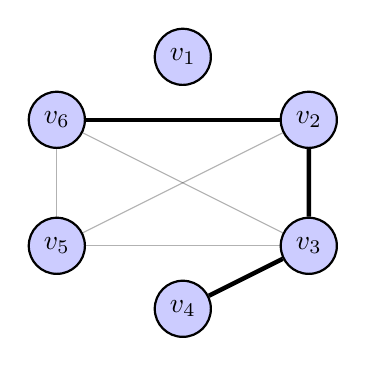
\begin{tikzpicture}
  [scale=.8,auto=left,every node/.style={circle,fill=blue!20,draw=black,thick}]
  \node (n1) at (2,4) {$v_1$};
  \node (n2) at (4,3)  {$v_2$};
  \node (n3) at (4,1)  {$v_3$};
  \node (n4) at (2,0) {$v_4$};
  \node (n5) at (0,1)  {$v_5$};
  \node (n6) at (0,3)  {$v_6$};

  \foreach \from/\to in {n3/n4,n2/n3, n2/n5, n2/n6, n3/n5, n3/n6, n5/n6}
  \draw[opacity=0.3] (\from) -- (\to);

  \foreach \from/\to in {n6/n2, n2/n3, n3/n4}
  \draw[ultra thick] (\from) -- (\to);

%\draw[ultra thick, red] (n2) -- (n6);
\end{tikzpicture}
}
        \caption{Un camino entre $v_6$ y $v_4$}
      \end{figure}
      \item En el grafo $G_1$ del \Cref{Ejm:Contenencia}, los vértices $v_4$ y $v_7$ están conectados por el camino $v_4v_5v_7$, pero $v_2$ y $v_6$ no están conectados por un camino.
      \begin{figure}[H]
        \centering
          \resizebox{0.3\textwidth}{!}{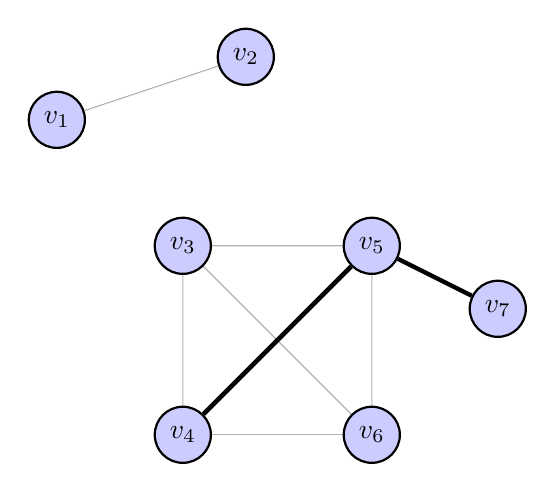
\begin{tikzpicture}
  [scale=.8,auto=left,every node/.style={circle,fill=blue!20,draw=black,thick}]
  \node (n1) at (0,5) {$v_1$};
  \node (n2) at (3,6) {$v_2$};
  \node (n3) at (2,3) {$v_3$};
  \node (n4) at (2,0) {$v_4$};
  \node (n5) at (5,3) {$v_5$};
  \node (n6) at (5,0) {$v_6$};
  \node (n7) at (7,2) {$v_7$};

  \foreach \from/\to in {n1/n2, n3/n5, n5/n6, n6/n4, n4/n3, n3/n6, n4/n5, n5/n7}
  \draw[opacity=0.3] (\from) -- (\to);


  \foreach \from/\to in {n4/n5, n5/n7}
  \draw[ultra thick] (\from) -- (\to);
\end{tikzpicture}
}
        \caption{Un camino entre $v_4$ y $v_7$}
      \end{figure}
   \end{itemize}
\end{Ejm}
\begin{Def}
   Un grafo $G$ es llamado \textbf{conexo} si $G\neq \emptyset$ y cualesquiera par de vértices  de $G$ están conectados por un camino en $G$. Si $G$ no es conexo, decimos que es \textbf{disconexo}. 
\end{Def}
Así, en el \Cref{Ejm:cuatro_grafos}, los grafos $G_1$, $G_3$ y $G_5$ son conexos, mientras que $G_2$ y $G_4$ son disconexos. Los grafos con un solo vértice son conexos.
\begin{Def}
   Sea $G$ un grafo. Un subgrafo conexo maximal de $G$ es llamado una \textbf{componente} de $G$. 
\end{Def}
Lo anterior nos quiere decir que un subgrafo $H\subseteq G$ es una componente de $G$ si y sólo si $H$ es conexo y además $H$ no está propiamente contenido en otro subgrafo conexo de $G$. Naturalmente, un grafo es conexo si y sólo si tiene una única componente. Además, como los grafos conexos son no vacíos, se sigue que el grafo vacío no tiene componentes.
\begin{Ejm}
   En los siguientes grafos se encierra con una línea punteada cada una de sus componentes.
   \begin{figure}[H]
     \centering
       \resizebox{0.45\textwidth}{!}{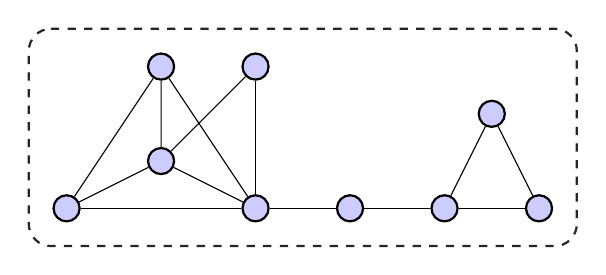
\begin{tikzpicture}[scale=.6,auto=left,every node/.style={circle,fill=blue!20,draw=black,thick}]
  \node (n1) at (0,0) {};
  \node (n2) at (2,3) {};
  \node (n3) at (2,1) {};
  \node (n4) at (4,3) {};
  \node (n5) at (4,0) {};
  \node (n6) at (6,0) {};
  \node (n7) at (8,0) {};
  \node (n8) at (9,2) {};
  \node (n9) at (10,0) {};
  
  \foreach \from/\to in {n1/n2,n1/n3,n1/n5,n2/n3,n2/n5,n3/n4,n3/n5,n4/n5,n5/n6,n6/n7,n7/n8,n7/n9,n8/n9}
    \draw (\from) -- (\to);

  % --- Envolvente estilo mano alzada para la componente conexa ---
  \begin{scope}[
    dashed,
    black!85,
    thick,
    decorate,
    decoration={random steps, segment length=5mm, amplitude=1.2mm}
  ]
    \draw[rounded corners=8pt] 
      (-0.8,3.8) -- (10.8,3.8) -- (10.8,-0.8) -- (-0.8,-0.8) -- cycle;
  \end{scope}

\end{tikzpicture}
}
     \caption{Un grafo con una componente}
   \end{figure}
   \begin{figure}[H]
     \centering
       \resizebox{0.35\textwidth}{!}{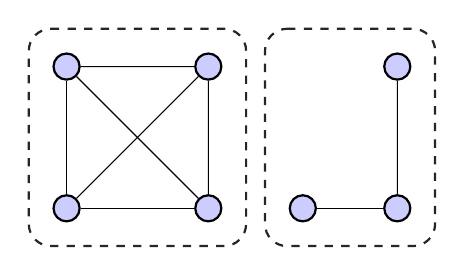
\begin{tikzpicture}
[scale=.6,auto=left,every node/.style={circle,fill=blue!20,draw=black,thick}]

  % Componente izquierda (Grafo completo K_4)
  \node (n1) at (0,3) {};
  \node (n2) at (3,3) {};
  \node (n3) at (0,0) {};
  \node (n4) at (3,0) {};

  \foreach \from/\to in {n1/n2,n1/n3,n1/n4,n2/n3,n2/n4,n3/n4}
    \draw (\from) -- (\to);

  % Componente derecha (Camino P_3)
  \node (n5) at (5,0) {};
  \node (n6) at (7,0) {};
  \node (n7) at (7,3) {};

  \foreach \from/\to in {n5/n6,n6/n7}
    \draw (\from) -- (\to);

  % --- Envolventes estilo mano alzada rectangulares ---
  \begin{scope}[
    dashed,
    black!85,
    thick,
    decorate,
    decoration={random steps, segment length=5mm, amplitude=1.2mm}
  ]
    % Envolvente izquierda (K_4)
    \draw[rounded corners=8pt] 
      (-0.8,3.8) -- (3.8,3.8) -- (3.8,-0.8) -- (-0.8,-0.8) -- cycle;

    % Envolvente derecha (P_3)
    \draw[rounded corners=8pt] 
      (4.2,3.8) -- (7.8,3.8) -- (7.8,-0.8) -- (4.2,-0.8) -- cycle;
  \end{scope}

\end{tikzpicture}
}
     \caption{Un grafo con dos componentes}
   \end{figure}
   \begin{figure}[H]
     \centering
       \resizebox{0.55\textwidth}{!}{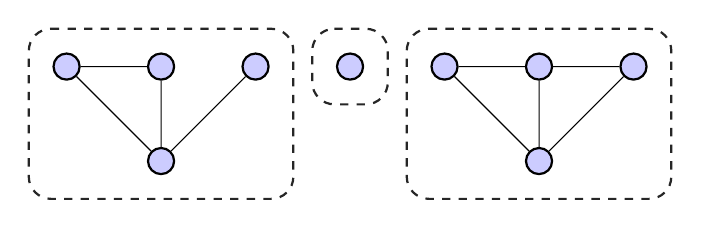
\begin{tikzpicture}
[scale=.6,auto=left,every node/.style={circle,fill=blue!20,draw=black,thick}]

  % Componente izquierda
  \node (n1) at (0,2) {};
  \node (n2) at (2,2) {};
  \node (n3) at (2,0) {};
  \node (n4) at (4,2) {};

  \foreach \from/\to in {n1/n2,n1/n3,n2/n3,n3/n4}
    \draw (\from) -- (\to);

  % Vértice aislado central
  \node (n5) at (6,2) {};

  % Componente derecha
  \node (n6) at (8,2) {};
  \node (n7) at (10,2) {};
  \node (n8) at (10,0) {};
  \node (n9) at (12,2) {};

  \foreach \from/\to in {n6/n7,n6/n8,n7/n8,n7/n9,n8/n9}
    \draw (\from) -- (\to);

  % --- Envolventes estilo mano alzada rectangulares ---
  \begin{scope}[
    dashed,
    black!85, % Color más oscuro
    thick,
    decorate,
    decoration={random steps, segment length=5mm, amplitude=1.2mm}
  ]
    % Envolvente izquierda (cuadrada/rectangular)
    \draw[rounded corners=8pt] 
      (-0.8,2.8) -- (4.8,2.8) -- (4.8,-0.8) -- (-0.8,-0.8) -- cycle;

    % Envolvente centro (alrededor de n5)
    \draw[rounded corners=8pt] 
      (5.2,2.8) -- (6.8,2.8) -- (6.8,1.2) -- (5.2,1.2) -- cycle;

    % Envolvente derecha (cuadrada/rectangular)
    \draw[rounded corners=8pt] 
      (7.2,2.8) -- (12.8,2.8) -- (12.8,-0.8) -- (7.2,-0.8) -- cycle;
  \end{scope}

\end{tikzpicture}
}
     \caption{Un grafo con tres componentes}
   \end{figure}
\end{Ejm}
Dado un grafo, se puede inducir un nuevo grafo al eliminar adecuadamente un subconjunto de vértices.
\begin{Def}
   Sean $G$ un grafo y $S\subseteq V(G)$. Denotamos por $\bm{G-S}$ al subgrafo de $G$ inducido por $V(G)\setminus S$, es decir, $G-S=G[V(G)\setminus S]$. 
\end{Def}\clearpage
\begin{Ejm}\label{Ejm:Supresion}
   \phantom{0}
   \begin{itemize}
      \item Si $S=\left\lbrace v_3,v_4\right\rbrace$ entonces:  
         \begin{figure}[H]
  \centering
  \resizebox{0.2\textwidth}{!}{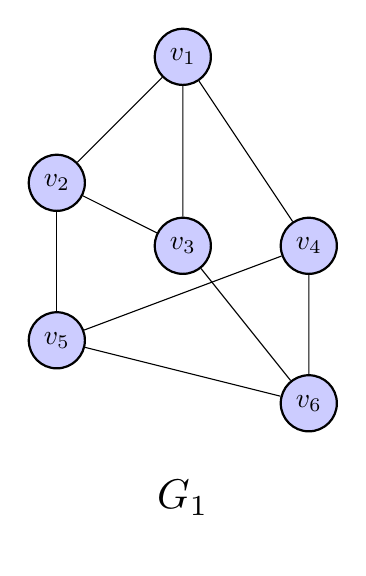
\begin{tikzpicture}
  [scale=.8,auto=left,every node/.style={circle,fill=blue!20,draw=black,thick}]
  \node (n1) at (3,6) {$v_1$};
  \node (n2) at (1,4) {$v_2$};
  \node (n3) at (3,3) {$v_3$};
  \node (n4) at (5,3) {$v_4$};
  \node (n5) at (1,1.5) {$v_5$};
  \node (n6) at (5,0.5) {$v_6$};

  \foreach \from/\to in {n1/n2, n1/n3, n1/n4, n2/n3, n2/n5, n3/n6, n4/n5, n4/n6, n5/n6}
    \draw (\from) -- (\to);

   \node[draw=none, fill=none, scale=1.5] at (3,-1) {$G_1$};
\end{tikzpicture}
} \hspace{2cm}
  \resizebox{0.2\textwidth}{!}{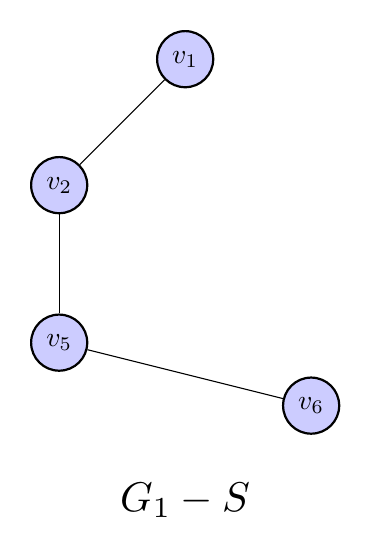
\begin{tikzpicture}
  [scale=.8,auto=left,every node/.style={circle,fill=blue!20,draw=black,thick}]
\useasboundingbox (0.5,-1.5) rectangle (5.5,6.5);
  \node (n1) at (3,6) {$v_1$};
  \node (n2) at (1,4) {$v_2$};
  \node (n3) at (3,3) [opacity=0]{$v_3$};
  \node (n4) at (5,3) [opacity=0]{$v_4$};
  \node (n5) at (1,1.5) {$v_5$};
  \node (n6) at (5,0.5) {$v_6$};

  \foreach \from/\to in {n1/n2, n2/n5, n5/n6}
    \draw (\from) -- (\to);

   \node[draw=none, fill=none, scale=1.5] at (3,-1) {$G_1-S$};
\end{tikzpicture}
} 
    \caption{$G_1$ y $G_1-S$}
\end{figure}
  
      \item Si $S'=\left\lbrace v_2,v_3,v_5\right\rbrace$ entonces:
         \vspace{1em}
         \par\vspace*{-5em}
{\centering
  \resizebox{0.23\textwidth}{!}{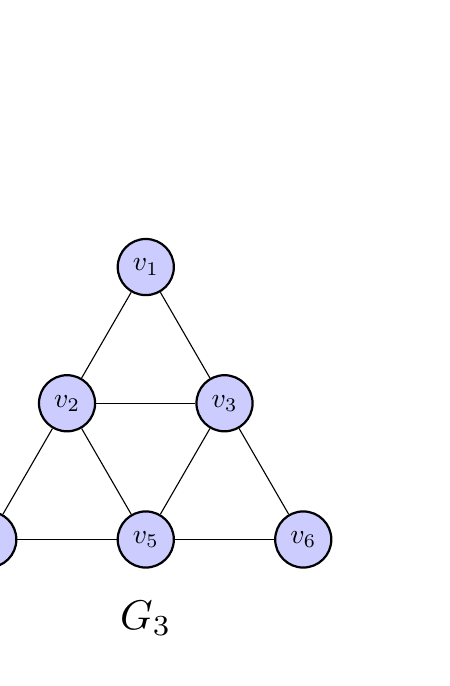
\begin{tikzpicture}
  [scale=1,auto=left,every node/.style={circle,fill=blue!20,draw=black,thick}]
\useasboundingbox (0.5,-1.5) rectangle (5.5,6.5);
  % Posiciones simétricas en forma de triángulo equilátero
  \node (n1) at (2,3.46) {$v_1$};
  \node (n2) at (1,1.73) {$v_2$};
  \node (n3) at (3,1.73) {$v_3$};
  \node (n4) at (0,0)    {$v_4$};
  \node (n5) at (2,0)    {$v_5$};
  \node (n6) at (4,0)    {$v_6$};

  % Aristas del grafo base (malla triangular)
  \foreach \from/\to in {n1/n2, n1/n3, n2/n3, n2/n4, n2/n5, n3/n5, n3/n6, n4/n5, n5/n6}
    \draw (\from) -- (\to);

   \node[draw=none, fill=none, scale=1.5] at (2,-1) {$G_3$};
\end{tikzpicture}
}%
  \hspace{2cm}%
  \resizebox{0.23\textwidth}{!}{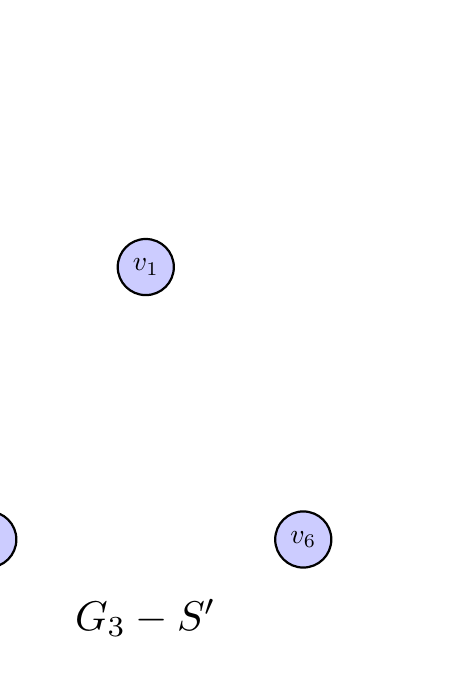
\begin{tikzpicture}
  [scale=1,auto=left,every node/.style={circle,fill=blue!20,draw=black,thick}]
\useasboundingbox (0.5,-1.5) rectangle (5.5,6.5); 
% Posiciones simétricas en forma de triángulo equilátero
  \node (n1) at (2,3.46) {$v_1$};
  \node (n2) at (1,1.73) [opacity=0]{$v_2$};
  \node (n3) at (3,1.73) [opacity=0]{$v_3$};
  \node (n4) at (0,0)    {$v_4$};
  \node (n5) at (2,0)    [opacity=0]{$v_5$};
  \node (n6) at (4,0)    {$v_6$};

  % Aristas del grafo base (malla triangular)
  %\foreach \from/\to in {n1/n2, n1/n3, n2/n3, n2/n4, n2/n5, n3/n5, n3/n6, n4/n5, n5/n6}
   % \draw (\from) -- (\to);

   \node[draw=none, fill=none, scale=1.5] at (2,-1) {$G_3-S'$};
\end{tikzpicture}
}\par
  \vspace{0.3em}%
  \captionof{figure}{$G_3$ y $G_3-S'$}
\par}
\vspace{1em}
  
   \end{itemize}
\end{Ejm}
Como se ve con el grafo $G_3$ del \Cref{Ejm:Supresion}, la supresión de algunos vértices en un grafo puede aumentar su número de componentes. La siguiente definición trata de casos especiales donde se da esta situación.
\begin{Def}
   Sea $G$ un grafo. Decimos que $v\in V(G)$ es un \textbf{vértice de corte} de $G$ si $G-\left\lbrace v\right\rbrace$ tiene más componentes que $G$. Si $G$ es conexo, decimos que un subconjunto de vértices $C\subseteq V(G)$ es un \textbf{conjunto de corte} de $G$ si $G-C$ tiene más de una componente. Si además, ningún subconjunto propio de $C$ es un conjunto de corte de $G$, decimos que $C$ es un \textbf{conjunto de corte minimal} de $G$.  
\end{Def}
\begin{Ejm}
   \phantom{o}
   \begin{itemize}
      \item En el grafo $G_1$, $v_1$ es un vértice de corte, pues $G_1-\left\lbrace v_1\right\rbrace$ tiene cuatro componentes, mientras que $G_1$ tiene dos componentes.
         \begin{figure}[H]
  \centering
  \resizebox{0.35\textwidth}{!}{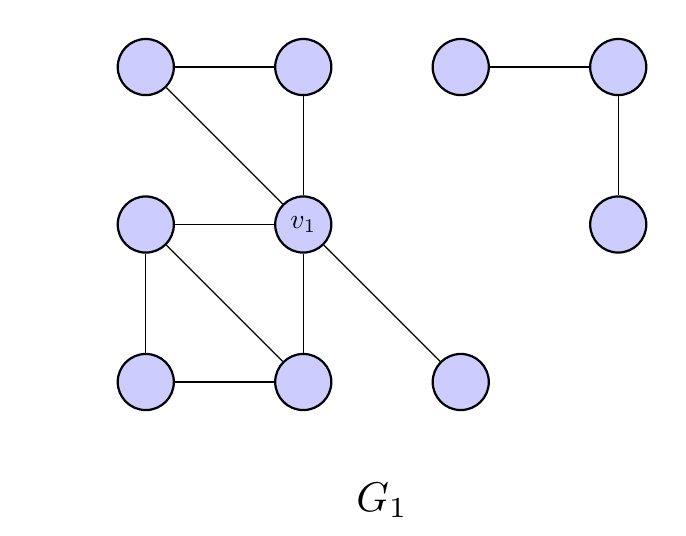
\begin{tikzpicture}[scale=1, auto=left, every node/.style={circle, fill=blue!20, draw=black, thick}]
    \node (v) at (3,2) {$v_1$};

  % Componente superior izquierda
    \node (u1) at (1,4) {\phantom{$v_1$}};
  \node (u2) at (3,4) {\phantom{$v_1$}};

  % Componente inferior izquierda
  \node (w1) at (1,2) {\phantom{$v_1$}};
  \node (w2) at (1,0) {\phantom{$v_1$}};
  \node (w3) at (3,0) {\phantom{$v_1$}};

  % Hoja inferior derecha
  \node (x1) at (5,0) {\phantom{$v_1$}};

  % Componente disjunta superior derecha
  \node (y1) at (5,4) {\phantom{$v_1$}};
  \node (y2) at (7,4) {\phantom{$v_1$}};
  \node (y3) at (7,2) {\phantom{$v_1$}};

  % Aristas
  \draw (u1) -- (u2);
  \draw (u1) -- (v);
  \draw (u2) -- (v);

  \draw (w1) -- (w2);
  \draw (w2) -- (w3);
  \draw (w1) -- (w3);
  \draw (w1) -- (v);
  \draw (w3) -- (v);

  \draw (v) -- (x1);

  \draw (y1) -- (y2);
  \draw (y2) -- (y3);

% Forzar Bounding Box idéntico en ambos diagramas
  \useasboundingbox (-0.5,-1.6) rectangle (7.5,4.5);
  % Etiqueta del grafo
  \node[draw=none, fill=none, scale=1.5] at (4,-1.5) {$G_1$};
\end{tikzpicture}
} \hspace{2cm}
  \resizebox{0.35\textwidth}{!}{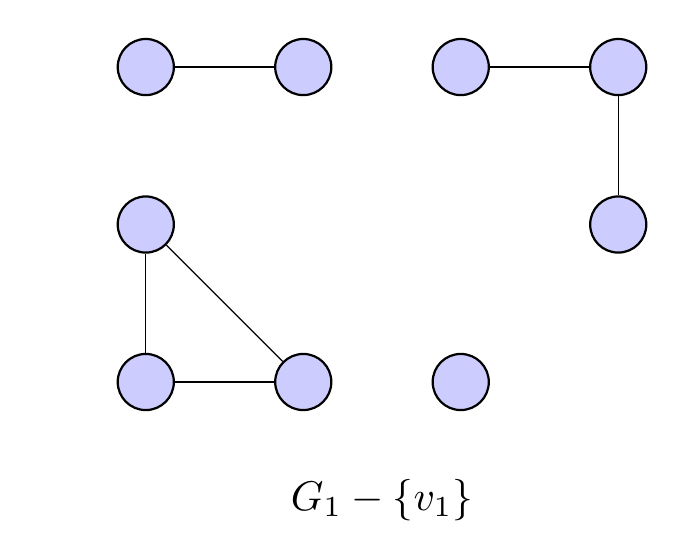
\begin{tikzpicture}[scale=1, auto=left, every node/.style={circle, fill=blue!20, draw=black, thick}]
  \node (v) at (3,2) [opacity=0]{$v_1$};

  % Componente superior izquierda
  \node (u1) at (1,4) {\phantom{$v_1$}};
  \node (u2) at (3,4) {\phantom{$v_1$}};

  % Componente inferior izquierda
  \node (w1) at (1,2) {\phantom{$v_1$}};
  \node (w2) at (1,0) {\phantom{$v_1$}};
  \node (w3) at (3,0) {\phantom{$v_1$}};

  % Hoja inferior derecha
  \node (x1) at (5,0) {\phantom{$v_1$}};

  % Componente disjunta superior derecha
  \node (y1) at (5,4) {\phantom{$v_1$}};
  \node (y2) at (7,4) {\phantom{$v_1$}};
  \node (y3) at (7,2) {\phantom{$v_1$}};

  % Aristas
  \draw (u1) -- (u2);

  \draw (w1) -- (w2);
  \draw (w2) -- (w3);
  \draw (w1) -- (w3);

  \draw (y1) -- (y2);
  \draw (y2) -- (y3);

% Forzar Bounding Box idéntico en ambos diagramas
  \useasboundingbox (-0.5,-1.6) rectangle (7.5,4.5);
  % Etiqueta del grafo
  \node[draw=none, fill=none, scale=1.5] at (4,-1.5) {$G_1-\left\lbrace v_1\right\rbrace$};
\end{tikzpicture}
} 
  \caption{Un vértice de corte}
\end{figure}
\vspace{-0.5cm}
      %\item En la siguiente figura, se tiene que $S:=\{u,v,w\}$ es un conjunto de corte del grafo conexo $G_2$, pues $G_2-S$ tiene dos componentes.\vspace{0.1cm}
      \item Tomemos $S=\{u,v,w\}$ y $S'=\{u,v\}$. En el grafo conexo $G_2$ que se muestra en la siguiente figura, $S$ es un conjunto de corte, pues $G_2-S$ tiene dos componentes.\vspace{0.1cm}
      \begin{figure}[H]
        \centering
        \resizebox{0.3\textwidth}{!}{\definecolor{customred}{HTML}{E7180B}

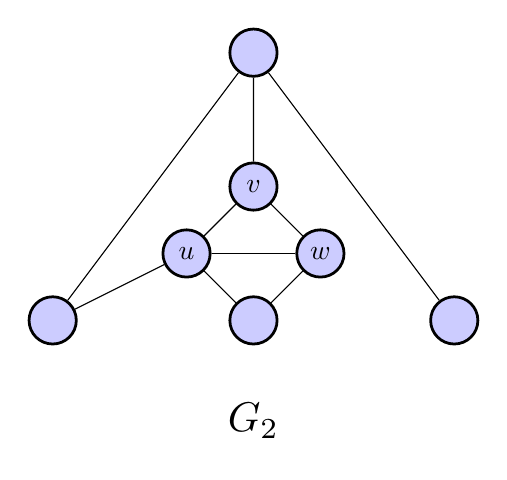
\begin{tikzpicture}[scale=0.85, auto=left]
  \tikzset{
    blue_node/.style={circle, fill=blue!20, draw, line width=1pt, inner sep=2pt, minimum size=6mm},
    red_node/.style={circle, fill=customred!20, draw=customred, line width=1pt, inner sep=2pt, minimum size=6mm}
  }

  % Vértices según la cuadrícula
  % Vértices con etiqueta
  \node[blue_node] (v) at (3,2) {$v$};
  \node[blue_node] (u) at (2,1) {$u$};
  \node[blue_node] (w) at (4,1) {$w$};

  % Vértices sin etiqueta (círculos vacíos)
  \node[blue_node] (top) at (3,4) {};
  \node[blue_node] (bottom) at (3,0) {};
  \node[blue_node] (left_bottom) at (0,0) {};
  \node[blue_node] (right_bottom) at (6,0) {};

  % Aristas del diamante interno (u, v, w, bottom)
  \draw (v) -- (u);
  \draw (v) -- (w);
  \draw (u) -- (w);
  \draw (u) -- (bottom);
  \draw (w) -- (bottom);

  % Conexiones del vértice superior (top)
  \draw (top) -- (v);
  \draw (top) -- (left_bottom);
  \draw (top) -- (right_bottom);

  % Conexión del vértice inferior izquierdo
  \draw (left_bottom) -- (u);

  % Bounding box para asegurar la alineación de la figura
  %\useasboundingbox (-0.5,-1.6) rectangle (6.5,6.5);

  % Etiqueta del grafo
  \node[draw=none, fill=none, scale=1.5] at (3,-1.5) {$G_2$};
\end{tikzpicture}
}\hspace{2cm}
        \resizebox{0.3\textwidth}{!}{\definecolor{customred}{HTML}{E7180B}

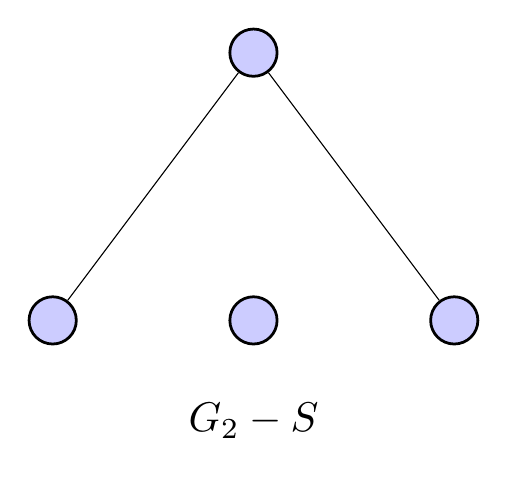
\begin{tikzpicture}[scale=0.85, auto=left]
  \tikzset{
    blue_node/.style={circle, fill=blue!20, draw, line width=1pt, inner sep=2pt, minimum size=6mm},
    red_node/.style={circle, fill=customred!20, draw=customred, line width=1pt, inner sep=2pt, minimum size=6mm}
  }

  % Vértices según la cuadrícula
  % Vértices con etiqueta
  \node[blue_node] (v) at (3,2) [opacity=0]{$v$};
  \node[blue_node] (u) at (2,1) [opacity=0]{$u$};
  \node[blue_node] (w) at (4,1) [opacity=0]{$w$};

  % Vértices sin etiqueta (círculos vacíos)
  \node[blue_node] (top) at (3,4) {};
  \node[blue_node] (bottom) at (3,0) {};
  \node[blue_node] (left_bottom) at (0,0) {};
  \node[blue_node] (right_bottom) at (6,0) {};

  % Aristas del diamante interno (u, v, w, bottom)

  % Conexiones del vértice superior (top)
  \draw (top) -- (left_bottom);
  \draw (top) -- (right_bottom);

  % Conexión del vértice inferior izquierdo

  % Bounding box para asegurar la alineación de la figura
  %\useasboundingbox (-0.5,-1.6) rectangle (6.5,6.5);

  % Etiqueta del grafo
  \node[draw=none, fill=none, scale=1.5] at (3,-1.5) {$G_2-S$};
\end{tikzpicture}
}
        \caption{$S$ es un conjunto de corte de $G_2$}
     \end{figure}\vspace{-0.4cm}
      Sin embargo $S$ no es un conjunto de corte minimal de $G_2$, ya que $S'\subsetneq S$ y $S'$ es un conjunto de corte de $G_2$, pues $G_2-S'$ tiene dos componentes.
      \begin{figure}[H]
        \centering
          \resizebox{0.3\textwidth}{!}{\definecolor{customred}{HTML}{E7180B}

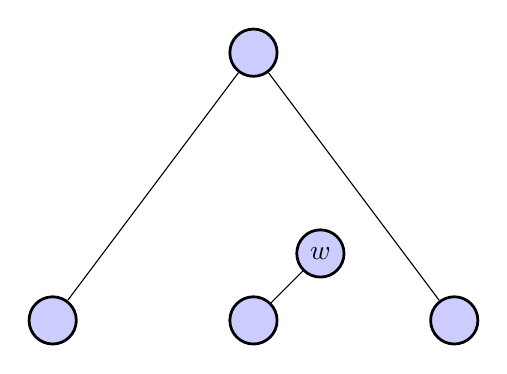
\begin{tikzpicture}[scale=0.85, auto=left]
  \tikzset{
    blue_node/.style={circle, fill=blue!20, draw, line width=1pt, inner sep=2pt, minimum size=6mm},
    red_node/.style={circle, fill=customred!20, draw=customred, line width=1pt, inner sep=2pt, minimum size=6mm}
  }

  % Vértices según la cuadrícula
  % Vértices con etiqueta
  \node[blue_node] (v) at (3,2) [opacity=0]{$v$};
  \node[blue_node] (u) at (2,1) [opacity=0]{$u$};
  \node[blue_node] (w) at (4,1) {$w$};

  % Vértices sin etiqueta (círculos vacíos)
  \node[blue_node] (top) at (3,4) {};
  \node[blue_node] (bottom) at (3,0) {};
  \node[blue_node] (left_bottom) at (0,0) {};
  \node[blue_node] (right_bottom) at (6,0) {};

  % Aristas del diamante interno (u, v, w, bottom)

  % Conexiones del vértice superior (top)
  \draw (top) -- (left_bottom);
  \draw (top) -- (right_bottom);
  \draw (w) -- (bottom);
  % Conexión del vértice inferior izquierdo

  % Bounding box para asegurar la alineación de la figura
  %\useasboundingbox (-0.5,-1.6) rectangle (6.5,6.5);

  % Etiqueta del grafo
  %\node[draw=none, fill=none, scale=1.5] at (3,-1.5) {$G_2-S'$};
\end{tikzpicture}
}
        \caption{El grafo $G_2-S'$}
      \end{figure}
      En cambio se tiene que $S'$ sí es un conjunto de corte minimal de $G_2$, pues ni $\{u\}$ ni $\{v\}$ son conjuntos de corte de $G_2$, ya que $G_2-\{u\}$ y $G_2-\{v\}$ son grafos conexos.\vspace{-1.2cm}
      \begin{figure}[H]
        \centering
           \resizebox{0.3\textwidth}{!}{\definecolor{customred}{HTML}{E7180B}

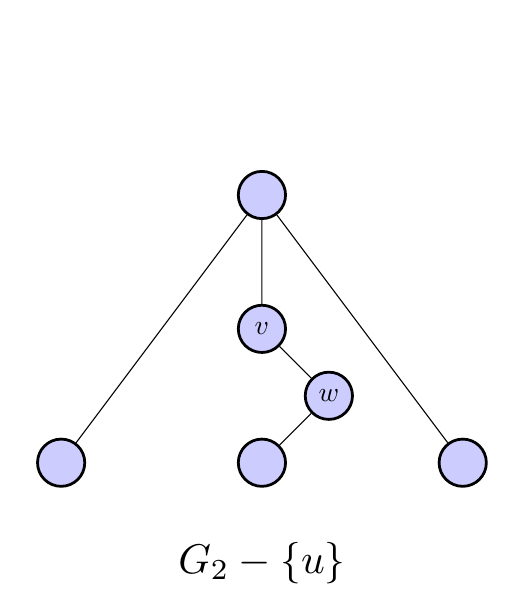
\begin{tikzpicture}[scale=0.85, auto=left]
  \tikzset{
    blue_node/.style={circle, fill=blue!20, draw, line width=1pt, inner sep=2pt, minimum size=6mm},
    red_node/.style={circle, fill=customred!20, draw=customred, line width=1pt, inner sep=2pt, minimum size=6mm}
  }

  % Vértices según la cuadrícula
  % Vértices con etiqueta
  \node[blue_node] (v) at (3,2) {$v$};
  \node[blue_node] (u) at (2,1) [opacity=0]{$u$};
  \node[blue_node] (w) at (4,1) {$w$};

  % Vértices sin etiqueta (círculos vacíos)
  \node[blue_node] (top) at (3,4) {};
  \node[blue_node] (bottom) at (3,0) {};
  \node[blue_node] (left_bottom) at (0,0) {};
  \node[blue_node] (right_bottom) at (6,0) {};

  % Aristas del diamante interno (u, v, w, bottom)
  \draw (v) -- (w);
  \draw (w) -- (bottom);

  % Conexiones del vértice superior (top)
  \draw (top) -- (v);
  \draw (top) -- (left_bottom);
  \draw (top) -- (right_bottom);

  % Conexión del vértice inferior izquierdo

  % Bounding box para asegurar la alineación de la figura
  \useasboundingbox (-0.5,-1.6) rectangle (6.5,6.5);

  % Etiqueta del grafo
  \node[draw=none, fill=none, scale=1.5] at (3,-1.5) {$G_2-\left\lbrace u\right\rbrace$};
\end{tikzpicture}
}\hspace{2cm}
          \resizebox{0.3\textwidth}{!}{\definecolor{customred}{HTML}{E7180B}

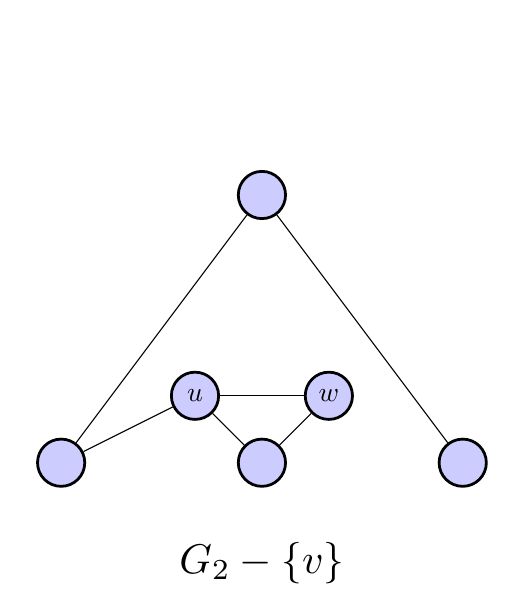
\begin{tikzpicture}[scale=0.85, auto=left]
  \tikzset{
    blue_node/.style={circle, fill=blue!20, draw, line width=1pt, inner sep=2pt, minimum size=6mm},
    red_node/.style={circle, fill=customred!20, draw=customred, line width=1pt, inner sep=2pt, minimum size=6mm}
  }

  % Vértices según la cuadrícula
  % Vértices con etiqueta
  \node[blue_node] (v) at (3,2) [opacity=0]{$v$};
  \node[blue_node] (u) at (2,1) {$u$};
  \node[blue_node] (w) at (4,1) {$w$};

  % Vértices sin etiqueta (círculos vacíos)
  \node[blue_node] (top) at (3,4) {};
  \node[blue_node] (bottom) at (3,0) {};
  \node[blue_node] (left_bottom) at (0,0) {};
  \node[blue_node] (right_bottom) at (6,0) {};

  % Aristas del diamante interno (u, v, w, bottom)
  \draw (u) -- (w);
  \draw (u) -- (bottom);
  \draw (w) -- (bottom);

  % Conexiones del vértice superior (top)
  \draw (top) -- (left_bottom);
  \draw (top) -- (right_bottom);

  % Conexión del vértice inferior izquierdo
  \draw (left_bottom) -- (u);

  % Bounding box para asegurar la alineación de la figura
  \useasboundingbox (-0.5,-1.6) rectangle (6.5,6.5);

  % Etiqueta del grafo
  \node[draw=none, fill=none, scale=1.5] at (3,-1.5) {$G_2-\left\lbrace v\right\rbrace$};
\end{tikzpicture}
}
          \vspace{0.5cm}
        \caption{Los grafos $G_2-\{u\}$ y $G_2-\{v\}$ son conexos}
      \end{figure}
   \end{itemize}
\end{Ejm}
\begin{Def}
   Sean $G$ un grafo y $S\subseteq V(G)$. Decimos que $S$ es \textbf{independiente} si para cualesquiera $u,v\in S$ se tiene $uv\notin E(G)$. En cambio, decimos que $S$ es un \textbf{clique} si para cualesquiera $u,v\in S$ se tiene $uv\in E(G)$.
\end{Def}
De esta forma, un subconjunto de vértices de un grafo es independiente si ningún par de estos vértices son adyacentes, y es un clique si cualquier par de estos vértices son adyacentes. En el \Cref{Ejm:cuatro_grafos}, $\left\lbrace v_2,v_4,v_6\right\rbrace$ es un conjunto independiente de $G_1$, $\left\lbrace v_1,v_2,v_3,v_4\right\rbrace$ es un clique de $G_2$, $\left\lbrace v_2,v_3,v_4,v_5,v_6\right\rbrace$ es un conjunto independiente de $G_3$ y $\left\lbrace v_2,v_3,v_5,v_6\right\rbrace$ es un clique de $G_4$.
\begin{Def}
   Dado un grafo $G=(V,E)$, su \textbf{complemento}, denotado $\overline{G}$, es el grafo con conjunto de vértices $V$ y conjunto de aristas $[V]^2\setminus E$. 
\end{Def}
Así, $\overline{G}$ mantiene los vértices de $G$, pero dos vértice son adyacentes en $\overline{G}$ si y sólo si no son adyacentes en $G$.
\begin{Ejm}
   La siguiente figura muestra ejemplos de grafos y sus complementos.\clearpage
   \par\vspace{1.5em}
{\centering
 % Fila superior (Diag33 y Diag34)
 \makebox[0.3\textwidth]{\resizebox{0.2\textwidth}{!}{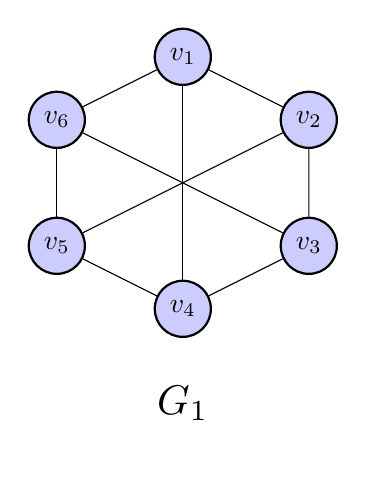
\begin{tikzpicture}
  [scale=.8,auto=left,every node/.style={circle,fill=blue!20,draw=black,thick}]
  \node (n1) at (2,4) {$v_1$};
  \node (n2) at (4,3)  {$v_2$};
  \node (n3) at (4,1)  {$v_3$};
  \node (n4) at (2,0) {$v_4$};
  \node (n5) at (0,1)  {$v_5$};
  \node (n6) at (0,3)  {$v_6$};

  \foreach \from/\to in {n1/n2,n2/n3,n3/n4,n4/n5,n5/n6,n6/n1,n6/n3,n1/n4,n2/n5}
    \draw (\from) -- (\to);

  % Etiqueta G_1 debajo del grafo
  \node[draw=none, fill=none, scale=1.5] at (2,-1.5) {$G_1$};

\end{tikzpicture}
}}%
 \hspace{2cm}%
 \makebox[0.3\textwidth]{\resizebox{0.2\textwidth}{!}{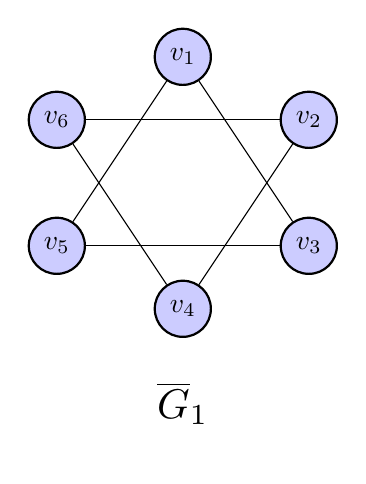
\begin{tikzpicture}
  [scale=.8,auto=left,every node/.style={circle,fill=blue!20,draw=black,thick}]
  \node (n1) at (2,4) {$v_1$};
  \node (n2) at (4,3) {$v_2$};
  \node (n3) at (4,1) {$v_3$};
  \node (n4) at (2,0) {$v_4$};
  \node (n5) at (0,1) {$v_5$};
  \node (n6) at (0,3) {$v_6$};

  % Aristas del complemento \overline{G}_1
  % Aristas rectas
  \draw (n1) -- (n3);
  \draw (n1) -- (n5);
  \draw (n2) -- (n4);
  \draw (n2) -- (n6);
  \draw (n3) -- (n5);
  \draw (n4) -- (n6);

  % Etiqueta \overline{G}_1 debajo del grafo
  \node[draw=none, fill=none, scale=1.5] at (2,-1.5) {$\overline{G}_1$};
\end{tikzpicture}
}}\par
 \vspace{0.5em}%
 % Fila inferior (Diag35 y Diag36)
 \makebox[0.3\textwidth]{\resizebox{0.25\textwidth}{!}{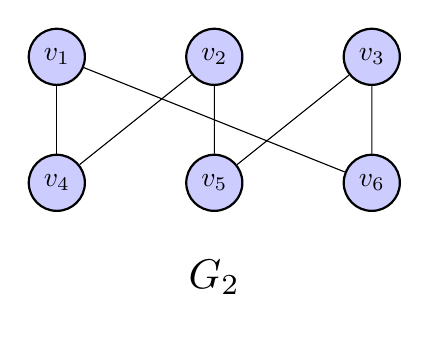
\begin{tikzpicture}
  [scale=.8,auto=left,every node/.style={circle,fill=blue!20,draw=black,thick}]
  
  % Fila superior (equivalente a la columna izquierda original)
  \node (n1) at (0,2) {$v_1$};
  \node (n2) at (2.5,2) {$v_2$};
  \node (n3) at (5,2) {$v_3$};

  % Fila inferior (equivalente a la columna derecha original)
  \node (n4) at (0,0) {$v_4$};
  \node (n5) at (2.5,0) {$v_5$};
  \node (n6) at (5,0) {$v_6$};

  % Aristas correspondientes a la imagen original
  \foreach \from/\to in {n1/n4, n1/n6, n2/n4, n2/n5, n3/n5, n3/n6}
    \draw (\from) -- (\to);

  % Etiqueta G_2 debajo del grafo
  \node[draw=none, fill=none, scale=1.5] at (2.5,-1.5) {$G_2$};

\end{tikzpicture}
}}%
 \hspace{2cm}%
 \makebox[0.3\textwidth]{\resizebox{0.25\textwidth}{!}{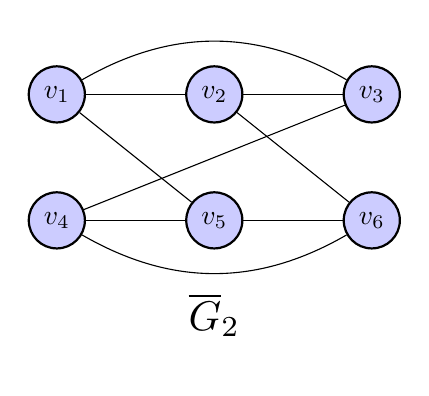
\begin{tikzpicture}
  [scale=.8,auto=left,every node/.style={circle,fill=blue!20,draw=black,thick}]
  
  % Fila superior
  \node (n1) at (0,2) {$v_1$};
  \node (n2) at (2.5,2) {$v_2$};
  \node (n3) at (5,2) {$v_3$};

  % Fila inferior
  \node (n4) at (0,0) {$v_4$};
  \node (n5) at (2.5,0) {$v_5$};
  \node (n6) at (5,0) {$v_6$};

  % Aristas del complemento \overline{G}_2
  % Conexiones dentro de la misma fila
  \draw (n1) to[bend left=30] (n3);
  \draw (n1) -- (n2);
  \draw (n2) -- (n3);
  
  \draw (n4) to[bend right=30] (n6);
  \draw (n4) -- (n5);
  \draw (n5) -- (n6);

  % Conexiones entre filas que faltaban en G_2
  \draw (n1) -- (n5);
  \draw (n2) -- (n6);
  \draw (n3) -- (n4);

  % Etiqueta \overline{G}_2 debajo del grafo
  \node[draw=none, fill=none, scale=1.5] at (2.5,-1.5) {$\overline{G}_2$};

\end{tikzpicture}
}}\par
 \captionof{figure}{Grafos y sus complementos}
\par}
\vspace{1em}

\end{Ejm}
Ahora procedemos a enunciar algunas clases especiales de grafos.
\begin{Def}
   Sea $G$ un grafo. Decimos que $G$ es \textbf{completo} si $V(G)$ es un clique. Un grafo completo con $n$ vértices se denota como $\bm{K^n}$.
\end{Def}
Por tanto, un grafo es completo si todos sus vértices son adyacentes dos a dos.
\begin{Ejm}
   El grafo vacío y el grafo con un solo vértice son grafos completos, que se denotan por $K^0$ y $K^1$, respectivamente. A continuación se muestran grafos completos con $3$, $5$ y $7$ vértices.
   \begin{figure}[H]
  \renewcommand{\diagscale}{0.2\textwidth}%
   \centering
   \resizebox{\diagscale}{!}{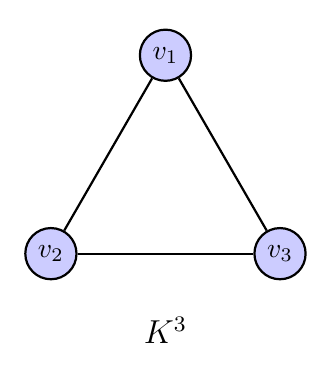
\begin{tikzpicture}[
  baseline=0pt,
  scale=0.7,
  vnode/.style={circle, draw=black, fill=blue!20, thick, inner sep=0pt, minimum size=6.5mm},
  edge/.style={thick, draw=black}
]
  \useasboundingbox (-2.5,-3.4) rectangle (2.5,2.3);

  % v1 en y=1.8, vértices inferiores en y=-1.8
  \node[vnode] (v1) at ([yshift=-0.6cm]90:2.4) {$v_1$};
  \node[vnode] (v2) at ([yshift=-0.6cm]210:2.4) {$v_2$};
  \node[vnode] (v3) at ([yshift=-0.6cm]330:2.4) {$v_3$};

  % Aristas
  \draw[edge] (v1) -- (v2);
  \draw[edge] (v2) -- (v3);
  \draw[edge] (v3) -- (v1);

  % Etiqueta
  \node[font=\large] at (0,-3.2) {$K^3$};
\end{tikzpicture}
}\hspace{4em}
   \resizebox{\diagscale}{!}{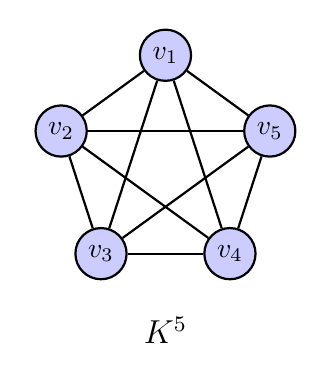
\begin{tikzpicture}[
  baseline=0pt,
  scale=0.7,
  vnode/.style={circle, draw=black, fill=blue!20, thick, inner sep=0pt, minimum size=6.5mm},
  edge/.style={thick, draw=black}
]
  \useasboundingbox (-2.5,-3.4) rectangle (2.5,2.3);

  % v1 en y=1.8, vértices inferiores en y=-1.8
  \node[vnode] (v1) at ([yshift=-0.19cm]90:1.99) {$v_1$};
  \node[vnode] (v2) at ([yshift=-0.19cm]162:1.99) {$v_2$};
  \node[vnode] (v3) at ([yshift=-0.19cm]234:1.99) {$v_3$};
  \node[vnode] (v4) at ([yshift=-0.19cm]306:1.99) {$v_4$};
  \node[vnode] (v5) at ([yshift=-0.19cm]18:1.99) {$v_5$};

  % Aristas
  \draw[edge] (v1) -- (v2); \draw[edge] (v1) -- (v3); \draw[edge] (v1) -- (v4); \draw[edge] (v1) -- (v5);
  \draw[edge] (v2) -- (v3); \draw[edge] (v2) -- (v4); \draw[edge] (v2) -- (v5);
  \draw[edge] (v3) -- (v4); \draw[edge] (v3) -- (v5);
  \draw[edge] (v4) -- (v5);

  % Etiqueta
  \node[font=\large] at (0,-3.2) {$K^5$};
\end{tikzpicture}
}\hspace{4em}
   \resizebox{\diagscale}{!}{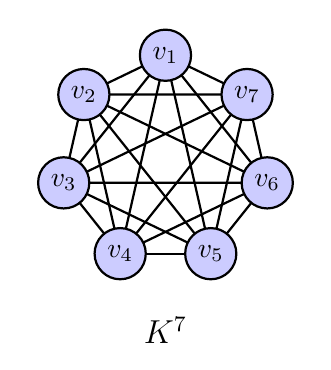
\begin{tikzpicture}[
  baseline=0pt,
  scale=0.7,
  vnode/.style={circle, draw=black, fill=blue!20, thick, inner sep=0pt, minimum size=6.5mm},
  edge/.style={thick, draw=black}
]
  \useasboundingbox (-2.5,-3.4) rectangle (2.5,2.3);

  \begin{scope}[yshift=-0.094cm]
    % Coordenadas con ángulos exactos
    \foreach \i in {1,...,7} {
      \pgfmathsetmacro{\ang}{90 + (\i-1)*360/7}
      \coordinate (v\i) at (\ang:1.894);
    }

    % Aristas
    \foreach \i in {1,...,6} {
      \pgfmathtruncatemacro{\start}{\i+1}
      \foreach \j in {\start,...,7} {
        \draw[edge] (v\i) -- (v\j);
      }
    }

    % Vértices
    \foreach \i in {1,...,7} {
      \node[vnode] at (v\i) {$v_\i$};
    }
  \end{scope}

  % Etiqueta
  \node[font=\large] at (0,-3.2) {$K^7$};
\end{tikzpicture}
}\vspace{0.5em}
 \caption{Ejemplos de grafos completos}
\end{figure}

\end{Ejm}
Para introducir los grafos conocidos como \textit{ciclos}, primero damos la siguiente definición.
\begin{Def}
   Sean $G$ un grafo y $F\subseteq [V(G)]^2$. Definimos el nuevo grafo $\bm{G+F}:=(V,E\cup F)$.
\end{Def}
De esta manera, lo que hacemos es adicionar a $G$, como nuevas aristas, las parejas de vértices que contenga $F$.
\begin{Ejm}
   \phantom{0}
   \begin{itemize}
      \item Si $F=\left\lbrace \left\lbrace v_2,v_6\right\rbrace, \left\lbrace v_2,v_5\right\rbrace, \left\lbrace v_3,v_6\right\rbrace, \left\lbrace v_3,v_5\right\rbrace\right\rbrace$ entonces:  
         \begin{figure}[H]
  \centering
  \resizebox{0.2\textwidth}{!}{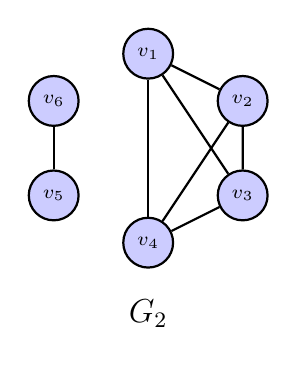
\begin{tikzpicture}
  [scale=.6, auto=left, 
   vertex/.style={circle, fill=blue!20, draw=black, thick, inner sep=2pt, minimum size=18pt},
   edge/.style={thick, draw=black}]

  % Vértices
  \node[vertex] (n1) at (2,4) {$\scriptstyle v_1$};
  \node[vertex] (n2) at (4,3) {$\scriptstyle v_2$};
  \node[vertex] (n3) at (4,1) {$\scriptstyle v_3$};
  \node[vertex] (n4) at (2,0) {$\scriptstyle v_4$};
  \node[vertex] (n5) at (0,1) {$\scriptstyle v_5$};
  \node[vertex] (n6) at (0,3) {$\scriptstyle v_6$};

  % Aristas del grafo base G_2
  \foreach \from/\to in {n1/n2, n2/n3, n1/n3, n1/n4, n2/n4, n3/n4, n5/n6}
    \draw[edge] (\from) -- (\to);

  % Etiqueta inferior
    \node at (2,-1.5) {\large{$G_2$}};
\end{tikzpicture}
} \hspace{2cm}
  \resizebox{0.2\textwidth}{!}{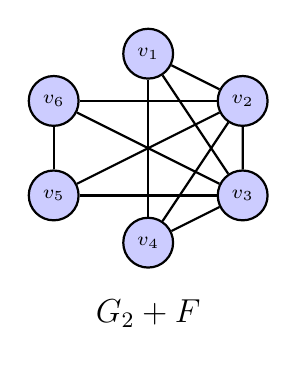
\begin{tikzpicture}
  [scale=.6, auto=left, 
   vertex/.style={circle, fill=blue!20, draw=black, thick, inner sep=2pt, minimum size=18pt},
   edge/.style={thick, draw=black},
   bold_edge/.style={line width=2.5pt, draw=black}]

  % Vértices
  \node[vertex] (n1) at (2,4) {$\scriptstyle v_1$};
  \node[vertex] (n2) at (4,3) {$\scriptstyle v_2$};
  \node[vertex] (n3) at (4,1) {$\scriptstyle v_3$};
  \node[vertex] (n4) at (2,0) {$\scriptstyle v_4$};
  \node[vertex] (n5) at (0,1) {$\scriptstyle v_5$};
  \node[vertex] (n6) at (0,3) {$\scriptstyle v_6$};

  % Aristas normales de G_2
  \foreach \from/\to in {n1/n2, n2/n3, n1/n3, n1/n4, n2/n4, n3/n4, n5/n6}
    \draw[edge] (\from) -- (\to);

  % Aristas reteñidas de F: {v3,v6}, {v3,v5}, {v2,v6}, {v2,v5}
  \foreach \from/\to in {n3/n6, n3/n5, n2/n6, n2/n5}
    \draw[edge] (\from) -- (\to);

  % Etiqueta inferior
    \node at (2,-1.5) {\large{$G_2 + F$}};
\end{tikzpicture}
} 
    \caption{$G_2$ y $G_2+F$}
\end{figure}
  
      \item Si $F'=\left\lbrace \left\lbrace v_2,v_3\right\rbrace, \left\lbrace v_3,v_4\right\rbrace, \left\lbrace v_4,v_5\right\rbrace, \left\lbrace v_5,v_6 \right\rbrace\right\rbrace$ entonces:
         \vspace{1em}
         \begin{figure}[H]
  \centering
  \resizebox{0.2\textwidth}{!}{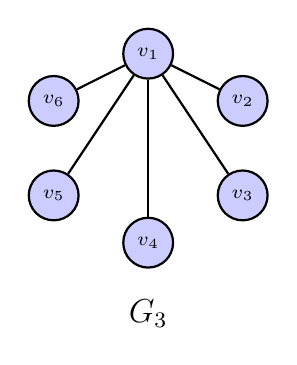
\begin{tikzpicture}
  [scale=.6, auto=left, 
   vertex/.style={circle, fill=blue!20, draw=black, thick, inner sep=2pt, minimum size=18pt},
   edge/.style={thick, draw=black}]

  % Vértices
  \node[vertex] (n1) at (2,4) {$\scriptstyle v_1$};
  \node[vertex] (n2) at (4,3) {$\scriptstyle v_2$};
  \node[vertex] (n3) at (4,1) {$\scriptstyle v_3$};
  \node[vertex] (n4) at (2,0) {$\scriptstyle v_4$};
  \node[vertex] (n5) at (0,1) {$\scriptstyle v_5$};
  \node[vertex] (n6) at (0,3) {$\scriptstyle v_6$};

  % Aristas del grafo G_3
  \foreach \from/\to in {n1/n2, n1/n3, n1/n4, n1/n5, n1/n6}
    \draw[edge] (\from) -- (\to);

  % Etiqueta inferior
    \node at (2,-1.5) {\large{$G_3$}};
\end{tikzpicture}
} \hspace{2cm}
  \resizebox{0.2\textwidth}{!}{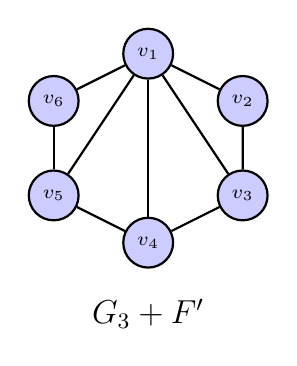
\begin{tikzpicture}
  [scale=.6, auto=left, 
   vertex/.style={circle, fill=blue!20, draw=black, thick, inner sep=2pt, minimum size=18pt},
   edge/.style={thick, draw=black}]

  % Vértices
  \node[vertex] (n1) at (2,4) {$\scriptstyle v_1$};
  \node[vertex] (n2) at (4,3) {$\scriptstyle v_2$};
  \node[vertex] (n3) at (4,1) {$\scriptstyle v_3$};
  \node[vertex] (n4) at (2,0) {$\scriptstyle v_4$};
  \node[vertex] (n5) at (0,1) {$\scriptstyle v_5$};
  \node[vertex] (n6) at (0,3) {$\scriptstyle v_6$};

  % Aristas originales de G_3
  \foreach \from/\to in {n1/n2, n1/n3, n1/n4, n1/n5, n1/n6}
    \draw[edge] (\from) -- (\to);

  % Aristas añadidas: {v2,v3}, {v3,v4}, {v4,v5}, {v5,v6}
  \foreach \from/\to in {n2/n3, n3/n4, n4/n5, n5/n6}
    \draw[edge] (\from) -- (\to);

  % Etiqueta inferior
    \node at (2,-1.5) {\large{$G_3+F'$}};
\end{tikzpicture}
} 
    \caption{$G_3$ y $G_3+F'$}
\end{figure}
  
   \end{itemize}
\end{Ejm}
\begin{Def}
   Sea $P=x_0\dots x_{k-1}$ un camino, con $k\geq 3$. Decimos que el grafo $C:=P+\left\lbrace \left\lbrace x_{k-1}, x_0\right\rbrace\right\rbrace$ es llamado un \textbf{ciclo}. En este caso denotamos a $C$ mediante $x_0x_1\dots x_{k-1}x_0$. La \textbf{longitud} de un ciclo es su número de aristas (que es igual a su número de vértices). Un ciclo de longitud $k$ es llamado un $\bm{k-ciclo}$ y es denotado por $\bm{C^k}$. 
\end{Def}
\begin{Ejm}
   Se tiene que $C^3=K^3$; éste es el ciclo de menor longitud posible. A continuación mostramos los ciclos de longitud $4$, $6$ y $8$.
   \begin{figure}[H]
  \renewcommand{\diagscale}{0.2\textwidth}%
   \centering
   \resizebox{\diagscale}{!}{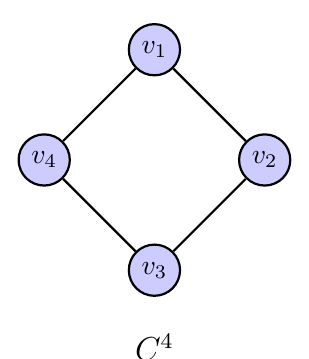
\begin{tikzpicture}[
  baseline=0pt,
  scale=0.7,
  vnode/.style={circle, draw=black, fill=blue!20, thick, inner sep=0pt, minimum size=6.5mm},
  edge/.style={thick, draw=black}
]
  \useasboundingbox (-2.3,-3.1) rectangle (2.3,2.4);

  % Vértices en radio 2.0 cm (v1 a 90°, v3 a 270°)
  \node[vnode] (v1) at (90:2.0) {$v_1$};
  \node[vnode] (v2) at (180:2.0) {$v_4$};
  \node[vnode] (v3) at (270:2.0) {$v_3$};
  \node[vnode] (v4) at (0:2.0) {$v_2$};

  % Aristas del ciclo C^4
  \draw[edge] (v1) -- (v2) -- (v3) -- (v4) -- (v1);

  % Etiqueta inferior en tamaño normal
  \node at (0,-3.4) {\large{$C^4$}};
\end{tikzpicture}
}\hspace{4em}
   \resizebox{\diagscale}{!}{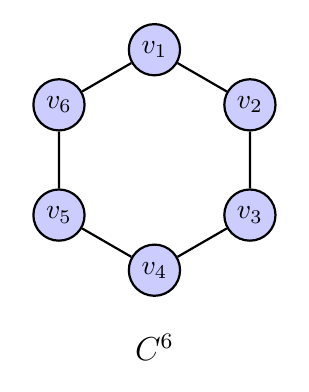
\begin{tikzpicture}[
  baseline=0pt,
  scale=0.7,
  vnode/.style={circle, draw=black, fill=blue!20, thick, inner sep=0pt, minimum size=6.5mm},
  edge/.style={thick, draw=black}
]
  \useasboundingbox (-2.3,-3.7) rectangle (2.3,2.4);

  % Vértices en radio 2.0 cm (v1 a 90°, aumentando en sentido horario)
  \foreach \i in {1,...,6} {
    \pgfmathsetmacro{\ang}{90 - (\i-1)*360/6}
    \node[vnode] (v\i) at (\ang:2.0) {$v_\i$};
  }

  % Aristas del ciclo C^6
  \draw[edge] (v1) -- (v2) -- (v3) -- (v4) -- (v5) -- (v6) -- (v1);

  % Etiqueta inferior en tamaño normal
  \node at (0,-3.4) {\large{$C^6$}};
\end{tikzpicture}
}\hspace{4em}
   \resizebox{\diagscale}{!}{\begin{tikzpicture}[
  baseline=0pt,
  scale=0.7,
  vnode/.style={circle, draw=black, fill=blue!20, thick, inner sep=0pt, minimum size=6.5mm},
  edge/.style={thick, draw=black}
]
  \useasboundingbox (-2.3,-3.7) rectangle (2.3,2.4);

  % Vértices en radio 2.0 cm (v1 a 90°, aumentando en sentido horario)
  \foreach \i in {1,...,8} {
    \pgfmathsetmacro{\ang}{90 - (\i-1)*360/8}
    \node[vnode] (v\i) at (\ang:2.0) {$v_\i$};
  }

  % Aristas del ciclo C^8
  \draw[edge] (v1) -- (v2) -- (v3) -- (v4) -- (v5) -- (v6) -- (v7) -- (v8) -- (v1);

  % Etiqueta inferior en tamaño normal
  \node at (0,-3.4) {\large{$C^8$}};
\end{tikzpicture}
}\vspace{1.3em}
 \caption{Ejemplos de ciclos}
\end{figure}

\end{Ejm}
Los ciclos nos permiten definir fácilmente lo que es un \textit{árbol}.
\begin{Def}
   Un grafo conexo que no contiene ningún ciclo es llamado un \textbf{árbol}. 
\end{Def}
\begin{Ejm}
   Todos los caminos son ejemplos de árboles. Los únicos grafos completos que son árboles son $K^1$ y $K^2$; el grafo $K^0=\emptyset$ no es un árbol porque no es conexo, y cualquier grafo completo con $3$ o más vértices contiene a $C^3$. En la \Cref{fig:arboles_ejemplos} los grafos $T_1$, $T_2$ y $T_3$ son ejemplos de árboles.
   \begin{figure}[H]
  \centering
  \begin{tikzpicture}[
  baseline=0pt,
  scale=1,
  vnode/.style={circle, draw=black, fill=blue!20, thick, inner sep=0pt, minimum size=4.5mm},
  edge/.style={thick, draw=black}
]
  \useasboundingbox (-2.3,-3.1) rectangle (2.3,2.4);

  % 4 vértices (Estrella / Tridente)
  \node[vnode] (v1) at (0, 1.8) {};     % Vértice superior
  \node[vnode] (v2) at (0, 0.0) {};     % Vértice central
  \node[vnode] (v3) at (-1.4, -1.8) {}; % Vértice inferior izq
  \node[vnode] (v4) at (1.4, -1.8) {};  % Vértice inferior der

  % Aristas
  \draw[edge] (v2) -- (v1);
  \draw[edge] (v2) -- (v3);
  \draw[edge] (v2) -- (v4);

  % Etiqueta
  \node[font=\large] at (0,-2.7) {$T_1$};
\end{tikzpicture}
\hfill
  \begin{tikzpicture}[
  baseline=0pt,
  scale=1,
  vnode/.style={circle, draw=black, fill=blue!20, thick, inner sep=0pt, minimum size=4.5mm},
  edge/.style={thick, draw=black}
]
  \useasboundingbox (-2.3,-3.1) rectangle (2.3,2.4);

  % Reflejos verticales manteniendo los límites y=-1.8 y y=1.8
  \begin{scope}[yscale=-1]
    \node[vnode] (v1) at (0.5, 1.8) {};
    \node[vnode] (v2) at (0.0, 1.2) {};
    \node[vnode] (v3) at (1.1, 1.4) {};
    \node[vnode] (v4) at (1.8, 1.7) {};
    \node[vnode] (v5) at (1.6, 0.9) {};
    \node[vnode] (v6) at (-0.7, 0.9) {};
    \node[vnode] (v7) at (0.2, 0.4) {};
    \node[vnode] (v8) at (-1.5, 1.3) {};
    \node[vnode] (v9) at (-1.6, 0.5) {};
    \node[vnode] (v10) at (-0.9, -0.1) {};
    \node[vnode] (v11) at (0.8, -0.2) {};
    \node[vnode] (v12) at (-0.1, -0.4) {};
    \node[vnode] (v13) at (1.5, -0.6) {};
    \node[vnode] (v14) at (0.9, -1.1) {};
    \node[vnode] (v15) at (-0.8, -1.0) {};
    \node[vnode] (v16) at (-0.1, -1.2) {};
    \node[vnode] (v17) at (-1.6, -1.5) {};
    \node[vnode] (v18) at (-0.8, -1.8) {};
    \node[vnode] (v19) at (0.0, -1.8) {};
    \node[vnode] (v20) at (0.8, -1.7) {};

    % Aristas
    \draw[edge] (v1) -- (v2); \draw[edge] (v1) -- (v3);
    \draw[edge] (v3) -- (v4); \draw[edge] (v3) -- (v5);
    \draw[edge] (v2) -- (v6); \draw[edge] (v2) -- (v7);
    \draw[edge] (v6) -- (v8); \draw[edge] (v6) -- (v9); \draw[edge] (v6) -- (v10);
    \draw[edge] (v7) -- (v11); \draw[edge] (v7) -- (v12);
    \draw[edge] (v11) -- (v13); \draw[edge] (v11) -- (v14);
    \draw[edge] (v12) -- (v15); \draw[edge] (v12) -- (v16);
    \draw[edge] (v15) -- (v17); \draw[edge] (v15) -- (v18);
    \draw[edge] (v16) -- (v19); \draw[edge] (v16) -- (v20);
  \end{scope}

  % Etiqueta
  \node[font=\large] at (0,-2.7) {$T_2$};
\end{tikzpicture}
\hfill
  \begin{tikzpicture}[
  baseline=0pt,
  scale=1,
  vnode/.style={circle, draw=black, fill=blue!20, thick, inner sep=0pt, minimum size=4.5mm},
  edge/.style={thick, draw=black}
]
  \useasboundingbox (-2.3,-3.1) rectangle (2.3,2.4);

  % Posicionamiento de los 13 vértices
  \node[vnode] (u1) at (-0.5, 1.8) {};   % Vértice superior
  \node[vnode] (u2) at (0.0, 1.2) {};
  \node[vnode] (u3) at (0.8, 1.6) {};
  \node[vnode] (u4) at (-0.8, 0.6) {};
  \node[vnode] (u5) at (-1.6, 0.9) {};
  \node[vnode] (u6) at (-0.2, 0.0) {};
  \node[vnode] (u7) at (0.6, -0.4) {};
  \node[vnode] (u8) at (1.4, -0.2) {};
  \node[vnode] (u9) at (1.2, -1.0) {};
  \node[vnode] (u10) at (-0.6, -0.7) {};
  \node[vnode] (u11) at (-1.4, -1.2) {};
  \node[vnode] (u12) at (-0.5, -1.8) {}; % Vértice inferior 1
  \node[vnode] (u13) at (0.5, -1.8) {};  % Vértice inferior 2

  % Aristas (12 conexiones)
  \draw[edge] (u2) -- (u1);
  \draw[edge] (u2) -- (u3);
  \draw[edge] (u2) -- (u4); \draw[edge] (u4) -- (u5);
  \draw[edge] (u2) -- (u6);
  \draw[edge] (u6) -- (u7); \draw[edge] (u7) -- (u8); \draw[edge] (u7) -- (u9);
  \draw[edge] (u6) -- (u10); \draw[edge] (u10) -- (u11); \draw[edge] (u10) -- (u12);
  \draw[edge] (u6) -- (u13);

  % Etiqueta
  \node[font=\large] at (0,-2.7) {$T_3$};
\end{tikzpicture}

  \caption{Ejemplos de árboles}
  \label{fig:arboles_ejemplos}
\end{figure}

   En la \Cref{fig:no_arboles}, el grafo $S_1$ no es un árbol porque no es conexo; el grafo $S_2$ no es un árbol porque contiene el ciclo $C^5$.
   \begin{figure}[H]
  \centering
  \begin{tikzpicture}[
  baseline=0pt,
  scale=1,
  vnode/.style={circle, draw=black, fill=blue!20, thick, inner sep=0pt, minimum size=4.5mm},
  edge/.style={thick, draw=black}
]
  \useasboundingbox (-2.3,-3.1) rectangle (2.3,2.4);

  % --- ÁRBOL 1 (10 vértices, trazado orgánico) ---
  \node[vnode] (t1_1) at (-1.2, 1.8) {};   % Vértice superior
  \node[vnode] (t1_2) at (-1.7, 1.1) {};
  \node[vnode] (t1_3) at (-0.7, 1.2) {};
  \node[vnode] (t1_4) at (-2.0, 0.3) {};
  \node[vnode] (t1_5) at (-1.3, 0.4) {};
  \node[vnode] (t1_6) at (-0.4, 0.5) {};
  \node[vnode] (t1_7) at (-1.6, -0.4) {};
  \node[vnode] (t1_8) at (-0.9, -0.3) {};
  \node[vnode] (t1_9) at (-1.8, -1.8) {};  % Vértice inferior
  \node[vnode] (t1_10) at (-1.0, -1.2) {};

  \draw[edge] (t1_1) -- (t1_2); \draw[edge] (t1_1) -- (t1_3);
  \draw[edge] (t1_2) -- (t1_4); \draw[edge] (t1_2) -- (t1_5);
  \draw[edge] (t1_3) -- (t1_6);
  \draw[edge] (t1_5) -- (t1_7); \draw[edge] (t1_5) -- (t1_8);
  \draw[edge] (t1_7) -- (t1_9); \draw[edge] (t1_8) -- (t1_10);

  % --- ÁRBOL 2 (5 vértices, trazado orgánico) ---
  \node[vnode] (t2_1) at (1.2, 1.1) {};
  \node[vnode] (t2_2) at (0.7, 0.2) {};
  \node[vnode] (t2_3) at (1.7, 0.3) {};
  \node[vnode] (t2_4) at (1.0, -0.7) {};
  \node[vnode] (t2_5) at (1.5, -1.8) {};   % Vértice inferior

  \draw[edge] (t2_2) -- (t2_1);
  \draw[edge] (t2_2) -- (t2_3);
  \draw[edge] (t2_2) -- (t2_4);
  \draw[edge] (t2_4) -- (t2_5);

  % Etiqueta
  \node[font=\large] at (0,-2.7) {$S_1$};
\end{tikzpicture}
\hspace{6em}
  \begin{tikzpicture}[
  baseline=0pt,
  scale=1,
  vnode/.style={circle, draw=black, fill=blue!20, thick, inner sep=0pt, minimum size=4.5mm},
  edge/.style={thick, draw=black},
  bold_edge/.style={line width=2.5pt, draw=black}
]
  \useasboundingbox (-2.3,-3.1) rectangle (2.3,2.4);

  % --- CICLO C^5 (Ubicado en la esquina inferior derecha) ---
  % c3 y c4 son los ÚNICOS dos vértices sin ramas adicionales (grado 2)
  \node[vnode] (c1) at (0.4, -0.5) {};   % Conecta con Rama 1 (Arriba-Izquierda)
  \node[vnode] (c2) at (1.2, -0.5) {};   % Conecta con Rama 2 (Arriba-Derecha)
  \node[vnode] (c3) at (1.7, -1.1) {};   % Vértice limpio (grado 2)
  \node[vnode] (c4) at (1.1, -1.8) {};   % Vértice limpio (grado 2, límite inferior)
  \node[vnode] (c5) at (0.3, -1.2) {};   % Conecta con Rama 3 (Abajo-Izquierda)

  % Aristas del C^5 (reteñidas)
  \draw[bold_edge] (c1) -- (c2) -- (c3) -- (c4) -- (c5) -- (c1);

  % --- RAMA 1: Sale de c5 (3 vértices hacia abajo/izquierda) ---
  \node[vnode] (v6) at (-0.4, -1.2) {};
  \node[vnode] (v7) at (-1.1, -1.8) {};  % Límite inferior
  \node[vnode] (v8) at (-0.3, -1.8) {};  % Límite inferior

  \draw[edge] (c5) -- (v6);
  \draw[edge] (v6) -- (v7);
  \draw[edge] (v6) -- (v8);

  % --- RAMA 2: Sale de c2 (3 vértices hacia la derecha/arriba) ---
  \node[vnode] (v9)  at (1.8, -0.1) {};
  \node[vnode] (v10) at (1.9, 0.6) {};
  \node[vnode] (v11) at (1.4, 1.2) {};

  \draw[edge] (c2) -- (v9);
  \draw[edge] (v9) -- (v10);
  \draw[edge] (v10) -- (v11);

  % --- RAMA 3: Sale de c1 (9 vértices hacia arriba e izquierda) ---
  \node[vnode] (v12) at (-0.3, 0.0) {};
  \node[vnode] (v13) at (-1.1, 0.2) {};
  \node[vnode] (v14) at (-1.7, 0.7) {};
  \node[vnode] (v15) at (-1.0, 0.8) {};
  \node[vnode] (v16) at (0.3, 0.6) {};
  \node[vnode] (v17) at (-0.3, 1.2) {};
  \node[vnode] (v18) at (-1.1, 1.6) {};
  \node[vnode] (v19) at (-0.4, 1.8) {};  % Límite superior
  \node[vnode] (v20) at (0.5, 1.8) {};   % Límite superior

  \draw[edge] (c1) -- (v12);
  \draw[edge] (v12) -- (v13);
  \draw[edge] (v13) -- (v14);
  \draw[edge] (v13) -- (v15);
  \draw[edge] (v12) -- (v16);
  \draw[edge] (v16) -- (v17);
  \draw[edge] (v17) -- (v18);
  \draw[edge] (v17) -- (v19);
  \draw[edge] (v16) -- (v20);

  % Etiqueta
  \node[font=\large] at (0,-2.7) {$S_2$};
\end{tikzpicture}

  \caption{Ejemplos de grafos que no son árboles}
  \label{fig:no_arboles}
\end{figure}

\end{Ejm}
\begin{Def}
   Sea $G$ un grafo de orden mayor o igual que $2$. Decimos que $G$ es \textbf{bipartito} si $V(G)$ admite una partición en dos clases $V_1$ y $V_2$ tales que $V_1$ y $V_2$ son conjuntos independientes. Si además cualesquiera dos vértices de distintas clases de la partición son adyacentes, decimos que $G$ es \textbf{bipartito completo}, y denotamos a $G$ por $K_{n_1,n_2}$, donde $n_1=|V_1|$ y $n_2=|V_2|$. Grafos de la forma $K_{1,n}$ con $n\in \mathbb{Z}^+$ son llamados \textbf{estrellas}.
\end{Def}
De esta forma, en un grafo bipartito con partición de vértices $\left\lbrace V_1,V_2\right\rbrace$, cada vértice de $V_1$ puede ser adyacente únicamente a vértices de $V_2$, y cada vértice de $V_2$ puede ser adyacente únicamente a vértices de $V_1$. Si el grafo es además bipartito completo, cada vértice de $V_1$ es adyacente a todos los vértices de $V_2$ (y por tanto cada vértice de $V_2$ es adyacente a todos los vértices de $V_1$).\\\\
Además, una estrella es un grafo con dos o más vértices en que un único vértice es adyacente a todos los demás, y las únicas aristas son las que permiten estas adyacencias.
\begin{Obs}
    Por convención, consideramos que el grafo vacío y el grafo $K^1$ son bipartitos. Esta precisión técnica es sumamente útil, pues evita tener que arrastrar condiciones de no trivialidad en los enunciados y demostraciones de teoremas en la teoría (por ejemplo, al caracterizar los grafos bipartitos como aquellos que no contienen ciclos de longitud impar, según la Proposición~1.6.1 de \cite{diestel2017}).
\end{Obs}
\begin{Ejm}
   La \Cref{fig:bipartitos_ejemplos} muestra el grafo bipartito $G_1$, que no es bipartito completo; el grafo bipartito completo $K_{3,5}$ y la estrella $K_{1,7}$. En cada grafo las respectivas particiones del conjunto de vértices son encerradas como en un diagrama de Venn.
   \begin{figure}[H]
  \centering
  \begin{tikzpicture}[
  baseline=0pt,
  scale=1,
  vnode/.style={circle, draw=black, fill=blue!20, thick, inner sep=0pt, minimum size=4.5mm},
  edge/.style={thick, draw=black}
]
  \useasboundingbox (-2.3,-3.1) rectangle (2.3,2.4);

  % Conjuntos de la partición (Venn)
  \draw[thick, draw=gray!70, fill=gray!10] (-1.2, 0) ellipse [x radius=0.65cm, y radius=2.15cm];
  \draw[thick, draw=gray!70, fill=gray!10] (1.2, 0) ellipse [x radius=0.65cm, y radius=2.15cm];

  % Vértices Partición Izquierda (3 vértices)
  \node[vnode] (a1) at (-1.2, 1.8) {};
  \node[vnode] (a2) at (-1.2, 0.0) {};
  \node[vnode] (a3) at (-1.2, -1.8) {}; % Tercer vértice (aislado)

  % Vértices Partición Derecha (4 vértices)
  \node[vnode] (b1) at (1.2, 1.8) {};
  \node[vnode] (b2) at (1.2, 0.6) {};
  \node[vnode] (b3) at (1.2, -0.6) {};
  \node[vnode] (b4) at (1.2, -1.8) {};

  % Aristas
  \draw[edge] (a1) -- (b1); 
  \draw[edge] (a1) -- (b2);
  \draw[edge] (a2) -- (b2); 
  \draw[edge] (a2) -- (b3); 
  \draw[edge] (a2) -- (b4); % Conexión añadida con el cuarto vértice de la derecha

  % Etiqueta inferior
  \node[font=\large] at (0,-2.7) {$G_1$};
\end{tikzpicture}
\hfill
  \begin{tikzpicture}[
  baseline=0pt,
  scale=1,
  vnode/.style={circle, draw=black, fill=blue!20, thick, inner sep=0pt, minimum size=4.5mm},
  edge/.style={thick, draw=black}
]
  \useasboundingbox (-2.3,-3.1) rectangle (2.3,2.4);

  % Conjuntos de la partición (Venn)
  \draw[thick, draw=gray!70, fill=gray!10] (-1.2, 0) ellipse [x radius=0.65cm, y radius=2.15cm];
  \draw[thick, draw=gray!70, fill=gray!10] (1.2, 0) ellipse [x radius=0.65cm, y radius=2.15cm];

  % Vértices Partición Izquierda (3 vértices)
  \node[vnode] (a1) at (-1.2, 1.8) {};
  \node[vnode] (a2) at (-1.2, 0.0) {};
  \node[vnode] (a3) at (-1.2, -1.8) {};

  % Vértices Partición Derecha (5 vértices)
  \node[vnode] (b1) at (1.2, 1.8) {};
  \node[vnode] (b2) at (1.2, 0.9) {};
  \node[vnode] (b3) at (1.2, 0.0) {};
  \node[vnode] (b4) at (1.2, -0.9) {};
  \node[vnode] (b5) at (1.2, -1.8) {};

  % Aristas (Todas las conexiones)
  \foreach \i in {1,2,3} {
    \foreach \j in {1,...,5} {
      \draw[edge] (a\i) -- (b\j);
    }
  }

  % Etiqueta inferior
  \node[font=\large] at (0,-2.7) {$K_{3,5}$};
\end{tikzpicture}
\hfill
  \begin{tikzpicture}[
  baseline=0pt,
  scale=1,
  vnode/.style={circle, draw=black, fill=blue!20, thick, inner sep=0pt, minimum size=4.5mm},
  edge/.style={thick, draw=black}
]
  \useasboundingbox (-2.3,-3.1) rectangle (2.3,2.4);

  % Partición 2 (Venn): Anillo exterior que encierra los 7 vértices
  \draw[thick, draw=gray!70, fill=gray!10, even odd rule] (0,0) circle (2.15cm) (0,0) circle (1.25cm);

  % Partición 1 (Venn): Círculo central que encierra el vértice central
  \draw[thick, draw=gray!70, fill=gray!10] (0,0) circle (0.65cm);

  % Vértice de la Partición 1 (Centro)
  \node[vnode] (a1) at (0, 0) {};

  % Vértices de la Partición 2 (7 vértices distribuidos uniformemente)
  \foreach \j in {1,...,7} {
    \pgfmathsetmacro{\ang}{90 + (\j-1)*360/7}
    \node[vnode] (b\j) at (\ang:1.8) {};
  }

  % Aristas desde el centro a cada vértice exterior
  \foreach \j in {1,...,7} {
    \draw[edge] (a1) -- (b\j);
  }

  % Etiqueta inferior
  \node[font=\large] at (0,-2.7) {$K_{1,7}$};
\end{tikzpicture}

  \caption{Ejemplos de grafos bipartitos}
  \label{fig:bipartitos_ejemplos}
\end{figure}

\end{Ejm}
La siguiente definición aborda el problema de la coloración de grafos.
\begin{Def}
   Sea $G$ un grafo. Una \textbf{coloración} de $G$ es una función $c: V(G) \to S$, donde $S$ es un conjunto cuyos elementos son llamados \textbf{colores}, tal que $c(u) \neq c(v)$ para cualesquiera dos vértices adyacentes $u, v \in V(G)$. Si el conjunto de colores $S$ tiene cardinalidad $k$, decimos que $c$ es una \textbf{$\bm{k}$-coloración}. Si $G$ tiene una \textbf{$\bm{k}$-coloración} decimos que $G$ es \textbf{$\bm{k}$-coloreable}. El menor cardinal $k$ para el cual existe una $k$-coloración de $G$ es el \textbf{número cromático} de $G$, el cual se denota por $\chi(G)$.
\end{Def}
Notemos que, para cualquier grafo $G$, la función identidad en $V(G)$ es una coloración de $G$; por tanto, todo grafo admite al menos una coloración y el número cromático $\chi(G)$ está bien definido. En particular, la función vacía de $\emptyset$ en $\emptyset$ es una coloración del grafo vacío, por lo que $\chi(\emptyset) = 0$. Para representar visualmente la coloración $c$ de un grafo, colocaremos la etiqueta correspondiente a $c(v)$ junto al círculo que representa al vértice $v$ (y no en su interior, para no confundirla con el vértice en sí). A continuación, mostramos algunos ejemplos de coloración de grafos.
\begin{Ejm}
   En la \Cref{tab:coloraciones_grafos}, para cada grafo $G_i$, con $i=1,2,3$, se tiene que $c_i$ es una coloración del grafo.
   \begin{longtable}{|S{c}|S{c}|S{c}|}
  % 1. DEFINIMOS EL PIE DE LA TABLA (AQUÍ VA EL CAPTION PARA QUE SALGA ABAJO)
  \hline
   \caption{Ejemplos de grafos con coloraciones}
  \addtocounter{table}{-1}\refstepcounter{table}% <-- Notifica a cleveref que es una tabla
  \label{tab:coloraciones_grafos} \\
  \endlastfoot
  
  % =========================================================
  % 2. A PARTIR DE AQUÍ VA EL CUERPO DE LA TABLA
  % =========================================================
  \hline
  % FILA 1: Nombres de los grafos
  \textbf{$G_1$} & \textbf{$G_2$} & \textbf{$G_3$} \\
  \hline
  
  % FILA 2: Grafos centrados en sus casillas
  \begin{tikzpicture}[
  baseline=0pt,
  scale=1,
  vnode/.style={circle, draw=black, fill=blue!20, thick, inner sep=0pt, minimum size=6.5mm},
  edge/.style={thick, draw=black},
  clabel/.style={font=\small, color=black}
]
  \useasboundingbox (-2.1,-2.3) rectangle (2.1,2.4);

  \begin{scope}[yshift=-0.2cm]
    % 7 Vértices
    \node[vnode, label={[clabel]above left:$1$}] (v1) at (0.0, 1.8) {$\scriptstyle v_1$};
    \node[vnode, label={[clabel]right:$2$}]        (v2) at (1.4, 0.9) {$\scriptstyle v_2$};
    \node[vnode, label={[clabel]right:$3$}]        (v3) at (1.4, -0.9) {$\scriptstyle v_3$};
    \node[vnode, label={[clabel]below:$4$}]        (v4) at (0.0, -1.8) {$\scriptstyle v_4$};
    \node[vnode, label={[clabel]left:$1$}]         (v5) at (-1.4, -0.9) {$\scriptstyle v_5$};
    \node[vnode, label={[clabel]left:$3$}]         (v6) at (-1.4, 0.9) {$\scriptstyle v_6$};
    \node[vnode, label={[clabel]above:$1$}]        (v7) at (0.0, 0.0) {$\scriptstyle v_7$};

    % Aristas
    \draw[edge] (v1) -- (v2) -- (v3) -- (v4) -- (v5) -- (v6) -- (v1);
    \draw[edge] (v7) -- (v2);
    \draw[edge] (v7) -- (v6);
    \draw[edge] (v7) -- (v4);
  \end{scope}
\end{tikzpicture}
 &
  \begin{tikzpicture}[
  baseline=0pt,
  scale=1,
  vnode/.style={circle, draw=black, fill=blue!20, thick, inner sep=0pt, minimum size=6.5mm},
  edge/.style={thick, draw=black},
  clabel/.style={font=\small, color=black}
]
  % Se amplía xmin a -2.55 para añadir el medio carácter de margen izquierdo
  \useasboundingbox (-2.55,-2.2) rectangle (2.25,2.3);

  \begin{scope}[yshift=-0.2cm]
    % --- COMPONENTE 1 ---
    \node[vnode, label={[clabel]above:$1$}] (v1) at (-1.2, 1.8) {$\scriptstyle v_1$};
    \node[vnode, label={[clabel]left:$2$}]  (v2) at (-1.8, 0.9) {$\scriptstyle v_2$};
    \node[vnode, label={[clabel]right:$3$}] (v3) at (-0.6, 0.9) {$\scriptstyle v_3$};
    \node[vnode, label={[clabel]left:$1$}]  (v4) at (-1.8, -0.4) {$\scriptstyle v_4$};
    \node[vnode, label={[clabel]right:$2$}] (v5) at (-0.6, -0.4) {$\scriptstyle v_5$};
    \node[vnode, label={[clabel]below:$3$}] (v6) at (-1.2, -1.8) {$\scriptstyle v_6$};

    \draw[edge] (v1) -- (v2) -- (v3) -- (v1);
    \draw[edge] (v2) -- (v4);
    \draw[edge] (v3) -- (v5);
    \draw[edge] (v4) -- (v5);
    \draw[edge] (v4) -- (v6);
    \draw[edge] (v5) -- (v6);

    % --- COMPONENTE 2 ---
    \node[vnode, label={[clabel]left:$1$}]  (v7)  at (1.2, 0.0) {$\scriptstyle v_7$};
    \node[vnode, label={[clabel]above:$2$}] (v8)  at (1.2, 1.8) {$\scriptstyle v_8$};
    \node[vnode, label={[clabel]below:$2$}] (v9)  at (0.5, -1.8) {$\scriptstyle v_9$};
    \node[vnode, label={[clabel]below:$2$}] (v10) at (1.9, -1.8) {$\scriptstyle v_{10}$};

    \draw[edge] (v7) -- (v8);
    \draw[edge] (v7) -- (v9);
    \draw[edge] (v7) -- (v10);
  \end{scope}
\end{tikzpicture}
 &
  \begin{tikzpicture}[
  baseline=0pt,
  scale=1,
  vnode/.style={circle, draw=black, fill=blue!20, thick, inner sep=0pt, minimum size=6.5mm},
  edge/.style={thick, draw=black},
  clabel/.style={font=\small, color=black}
]
  % Caja delimitadora simétrica (-1.8 a 1.8) para centrar el eje x = 0
  \useasboundingbox (-1.8,-2.8) rectangle (1.8,2.4);

  \begin{scope}[yshift=-0.2cm]
    % Primeros 5 vértices
    \node[vnode, label={[clabel]above:$1$}]        (v1) at (0.0, 1.8) {$\scriptstyle v_1$};
    \node[vnode, label={[clabel]left:$2$}]         (v2) at (-0.9, 0.9) {$\scriptstyle v_2$};
    \node[vnode, label={[clabel]right:$1$}]        (v3) at (0.9, 0.0) {$\scriptstyle v_3$};
    \node[vnode, label={[clabel]left:$2$}]         (v4) at (-0.9, -0.9) {$\scriptstyle v_4$};
    \node[vnode, label={[clabel]below left:$1$}] (v5) at (0.0, -1.8) {$\scriptstyle v_5$};

    % Aristas
    \draw[edge] (v1) -- (v2) -- (v3) -- (v4) -- (v5);
    \draw[edge] (v5) -- (1.2, -2.4);
    \node[font=\small] at (1.5, -2.4) {$\dots$};
  \end{scope}
\end{tikzpicture}
 \\
  \hline
  
  % FILA 3: Funciones alineadas
  $\begin{aligned}[t]
      c_1 \!:\phantom{o} V(G_1) &\to \{1, 2, 3, 4\} \\
     v_1 &\mapsto 1 \\
     v_2 &\mapsto 2 \\
     v_3 &\mapsto 3 \\
     v_4 &\mapsto 4 \\
     v_5 &\mapsto 1 \\
     v_6 &\mapsto 3 \\
     v_7 &\mapsto 1
  \end{aligned}$ 
  &
  $\begin{aligned}[t]
     c_2 \!:\phantom{o} V(G_2) &\to \{1, 2, 3\} \\
     v_1 &\mapsto 1 \\
     v_2 &\mapsto 2 \\
     v_3 &\mapsto 3 \\
     v_4 &\mapsto 1 \\
     v_5 &\mapsto 2 \\
     v_6 &\mapsto 3 \\
     v_7 &\mapsto 1 \\
     v_8 &\mapsto 2 \\
     v_9 &\mapsto 2 \\
     v_{10} &\mapsto 2
  \end{aligned}$ 
  &
  $\begin{aligned}[t]
     c_3 \!:\phantom{o} V(G_3) &\to \{1, 2\} \\
     v_i &\mapsto 
     \begin{cases} 
       1 & \begin{array}[t]{@{}l@{}} \text{si } i \text{ es} \\[-1ex] \text{impar} \end{array} \\[0.6ex]
       2 & \begin{array}[t]{@{}l@{}} \text{si } i \text{ es} \\[-1ex] \text{par} \end{array} 
     \end{cases}
  \end{aligned}$ \\
  \hline
\end{longtable}

\end{Ejm}
